\section{PLANIFICACIÓN DEL PROYECTO}
En este apartado se abordará la planificación inicial del proyecto, detallando los aspectos más relevantes del mismo. 
Se incluirá la identificación de interesados, las tareas a realizar, la estructura de desglose de trabajo, la planificación temporal, los riesgos identificados y el presupuesto inicial.

\subsection{Identificación de Interesados}
Los interesados en el proyecto son las personas o grupos que pueden afectar o verse afectados por el proyecto. 
En el caso de este proyecto, los interesados son los siguientes:
\begin{itemize}
    \item \textbf{Usuarios:} Compradores de sobres, vendedores en subastas, pujadores y coleccionistas. Su satisfacción y experiencia de usuario son críticas para el éxito de la plataforma.
    \item \textbf{Desarrolladores:} Equipo encargado del desarrollo, mantenimiento y actualización de la plataforma.
    \item \textbf{Propietarios/Creadores:} Fundadores y administradores del proyecto, responsables de la visión, dirección y toma de decisiones estratégicas.
    \item \textbf{Inversores:} Personas o entidades que financian el proyecto, con expectativas de retorno sobre su inversión. Su interés reside en la rentabilidad y sostenibilidad del negocio.
    \item \textbf{Proveedores:} Proveedores de servicios tecnológicos y de infraestructura, como \textit{hosting}, sistemas de pago y seguridad.
    \item \textbf{Comunidades:} Grupos y foros de fans y coleccionistas de Pokémon que pueden influir en la popularidad y adopción de la plataforma. Su participación y \textit{feedback} pueden guiar mejoras y nuevas características.
    \item \textbf{Reguladores:} Entidades gubernamentales y de la industria que aseguran el cumplimiento de leyes y regulaciones aplicables al comercio digital y la protección de datos.
\end{itemize}


\subsection{OBS y PBS}
El OBS, \textit{Organizational Breakdown Structure} es una estructura que representa las responsabilidades sobre la realización de las tareas del proyecto. 
Por otro lado, el PBS  \textit{(Product Breakdown Structure)} es una estructura jerárquica que descompone el proyecto en los productos que se deben entregar para cumplir con los objetivos del proyecto.

\subsubsection{OBS} \label{sec:5-OBS}
\hypertarget{sec:5-OBS}{}
En este proyecto, se simulará una pequeña empresa ficticia para su realización. 
Se han identificado los distintos perfiles que intervienen en el proyecto, así como las tareas que cada uno debe realizar. 
Aunque el proyecto se llevará a cabo de forma individual, se ha considerado necesario estructurar estos roles para poder asignar un presupuesto adecuado a cada función.

Los roles identificados se especifican en \coloredUnderline{\hyperlink{table:obs}{Tabla: \ref*{table:obs} \nameref*{table:obs}}}. 
Cabe destacar que el rol de Jefe de Proyecto (JP) es el encargado de supervisar y coordinar el trabajo de los demás roles y este rol ha sido considerado tanto para el alumno como para el tutor del TFG.


\begin{table}[H]
\centering
\hypertarget{table:obs}{}
\caption{OBS (Organizational Breakdown Structure)}
\label{table:obs}
\begin{tabular}{>{\columncolor{lightgreen!20}}p{7cm} p{10cm}}
\toprule
\rowcolor{darkgreen!50}
\textbf{Abreviatura} & \textbf{Rol} \\
\midrule
JP & Jefe de Proyecto \\
\midrule
AN & Analista junior\\
\midrule
DI & Diseñador junior \\
\midrule
DS & Desarrollador de Software junior\\
\midrule
TE & Tester junior \\
\midrule
DOC & Documentador técnico \\
\bottomrule
\end{tabular}
\end{table}
 
Se ha decidido realizar una matriz de asignación de responsabilidades RACI para relacionar las tareas identifcadas en \coloredUnderline{\hyperlink{sec:5-WBS}{\ref*{sec:5-WBS} \nameref*{sec:5-WBS}}} con cada rol.
En esta matriz, a cada tarea se le asigna un rol con una de las siguientes responsabilidades:
\begin{itemize}
    \item \textbf{R:} Responsable. Persona que realiza la tarea.
    \item \textbf{A:} Aprobador. Persona que aprueba la tarea.
    \item \textbf{C:} Consultado. Persona a la que se consulta sobre la tarea.
    \item \textbf{I:} Informado. Persona a la que se informa sobre el avance y los resultados de la tarea.
\end{itemize}
Un mismo recursos puede tener varias responsabilidades en una misma tarea, en tal caso se anotarán separadas por el caracter \textit{``/''}.

\subsubsubsection{Análisis del proyecto}
En la \coloredUnderline{\hyperlink{table:matriz-analisis}{Tabla: \ref*{table:matriz-analisis} \nameref*{table:matriz-analisis}}} se muestra la matriz de responsabilidades para la fase de análisis.
\begin{table}[H]
    \centering
    \caption{Matriz RACI. Análisis del proyecto}
    \label{table:matriz-analisis}
    \hypertarget{table:matriz-analisis}{}
    \begin{tabular}{
    >{\columncolor{lightgreen!20}}m{7cm} 
    >{\columncolor{white}}m{1cm} 
    >{\columncolor{white}}m{1cm} 
    >{\columncolor{white}}m{1cm} 
    >{\columncolor{white}}m{1cm} 
    >{\columncolor{white}}m{1cm} 
    >{\columncolor{white}}m{1cm}}
    \cmidrule(l){2-7}
    \rowcolor{darkgreen!50}
    \cellcolor{white} & \multicolumn{6}{c}{\textbf{Roles}} \\
    \midrule
    \rowcolor{lightgreen!20}
    \cellcolor{darkgreen!50}\textbf{Tarea} & \textbf{JP} & \textbf{AN} & \textbf{DI} & \textbf{DS} & \textbf{TE} & \textbf{DOC} \\
    \midrule
    Análisis del sistema & A & R &  & C &  &  \\
    \midrule
    Análisis de la arquitectura & A & R &  & C &  &  \\
    \midrule
    Análisis de la infraestructura & A & R &  & C &  &  \\
    \midrule
    Determinación del alcance de desarrollo & A & R & I & C & I & I \\
    \bottomrule
    \end{tabular}
\end{table}

\subsubsubsection{Seguimiento del proyecto}
En la \coloredUnderline{\hyperlink{table:matriz-seguimiento}{Tabla: \ref*{table:matriz-seguimiento} \nameref*{table:matriz-seguimiento}}} se muestra la matriz de responsabilidades para la fase de seguimiento.
\begin{table}[H]
    \centering
    \caption{Matriz RACI. Seguimiento del proyecto}
    \label{table:matriz-seguimiento}
    \hypertarget{table:matriz-seguimiento}{}
    \begin{tabular}{
    >{\columncolor{lightgreen!20}}m{7cm} 
    >{\columncolor{white}}m{1cm} 
    >{\columncolor{white}}m{1cm} 
    >{\columncolor{white}}m{1cm} 
    >{\columncolor{white}}m{1cm} 
    >{\columncolor{white}}m{1cm} 
    >{\columncolor{white}}m{1cm}}
    \cmidrule(l){2-7}
    \rowcolor{darkgreen!50}
    \cellcolor{white} & \multicolumn{6}{c}{\textbf{Roles}} \\
    \midrule
    \rowcolor{lightgreen!20}
    \cellcolor{darkgreen!50}\textbf{Tarea} & \textbf{JP} & \textbf{AN} & \textbf{DI} & \textbf{DS} & \textbf{TE} & \textbf{DOC} \\
    \midrule
    Reunión de arranque & A & I & I & I & I & R \\
    \midrule
    Reuniones periódicas & A & I & I & I & I & R\\
    \midrule
    Reunión de revisión & A & I & I & C & I & R  \\
    \midrule
    Reunión final & A & I & I & C & I & R  \\
    \bottomrule
    \end{tabular}
\end{table}

\subsubsubsection{Diseño del sistema}
En la \coloredUnderline{\hyperlink{table:matriz-diseno}{Tabla: \ref*{table:matriz-diseno} \nameref*{table:matriz-diseno}}} se presenta la matriz de responsabilidades correspondiente a la fase de diseño. 
Las tareas listadas en esta matriz son las tareas "hoja" de dicha fase, es decir, aquellas que no se descomponen en subtareas más pequeñas y, por lo tanto, representan las tareas finales 
de la fase de diseño.
\begin{table}[H]
    \centering
    \caption{Matriz RACI. Diseño del sistema}
    \label{table:matriz-diseno}
    \hypertarget{table:matriz-diseno}{}
    \begin{tabular}{
    >{\columncolor{lightgreen!20}}m{7cm} 
    >{\columncolor{white}}m{1cm} 
    >{\columncolor{white}}m{1cm} 
    >{\columncolor{white}}m{1cm} 
    >{\columncolor{white}}m{1cm} 
    >{\columncolor{white}}m{1cm} 
    >{\columncolor{white}}m{1cm}}
    \cmidrule(l){2-7}
    \rowcolor{darkgreen!50}
    \cellcolor{white} & \multicolumn{6}{c}{\textbf{Roles}} \\
    \midrule
    \rowcolor{lightgreen!20}
    \cellcolor{darkgreen!50}\textbf{Tarea} & \textbf{JP} & \textbf{AN} & \textbf{DI} & \textbf{DS} & \textbf{TE} & \textbf{DOC} \\
    \midrule
    \textit{Backend}. Diseño del módulo de usuarios & A &  & I & R &  &  I \\
    \midrule
    \textit{Backend}. Diseño del módulo de cartas & A &  & I & R &  & I \\
    \midrule
    \textit{Backend}. Diseño del módulo de sobres de cartas & A &  & I & R &  & I \\
    \midrule
    \textit{Backend}. Diseño del módulo de subastas & A &  & I & R &  & I \\
    \midrule
    \textit{Backend}. Diseño del módulo de transacciones & A &  & I & R &  & I \\
    \midrule
    \textit{Frontend}. Diseño de logo de la aplicación & A &  & R & I &  & I \\
    \midrule
    \textit{Frontend}. Diseño de la moneda de la aplicación & A &  & R & I &  & I \\
    \midrule
    \textit{Frontend}. Diseño de la temática & A &  & R & C/I &  & I \\
    \midrule
    \textit{Frontend}. Diseño del árbol de navegación & A &  & R & C/I &  & I \\
    \midrule
    \textit{Frontend}. Diseño de las páginas de información & A &  & R & C/I &  & I \\
    \midrule
    \textit{Frontend}. Diseño de las página \textit{Home} & A &  & R & C/I &  & I \\
    \midrule
    \textit{Frontend}. Diseño de las página de error & A &  & R & C/I &  & I \\
    \bottomrule
    \end{tabular}
\end{table}

\subsubsubsection{Implementación del sistema}
En la \coloredUnderline{\hyperlink{table:matriz-implementacion}{Tabla: \ref*{table:matriz-implementacion} \nameref*{table:matriz-implementacion}}} se muestra la matriz de responsabilidades para la fase de implementación.
\begin{table}[H]
    \centering
    \caption{Matriz RACI. Implementación del proyecto}
    \label{table:matriz-implementacion}
    \hypertarget{table:matriz-implementacion}{}
    \begin{tabular}{
    >{\columncolor{lightgreen!20}}m{7cm} 
    >{\columncolor{white}}m{1cm} 
    >{\columncolor{white}}m{1cm} 
    >{\columncolor{white}}m{1cm} 
    >{\columncolor{white}}m{1cm} 
    >{\columncolor{white}}m{1cm} 
    >{\columncolor{white}}m{1cm}}
    \cmidrule(l){2-7}
    \rowcolor{darkgreen!50}
    \cellcolor{white} & \multicolumn{6}{c}{\textbf{Roles}} \\
    \midrule
    \rowcolor{lightgreen!20}
    \cellcolor{darkgreen!50}\textbf{Tarea} & \textbf{JP} & \textbf{AN} & \textbf{DI} & \textbf{DS} & \textbf{TE} & \textbf{DOC} \\
    \midrule
    Reunión de arranque & A & I & I & I & I & R \\
    \midrule
    Reuniones periódicas & A & I & I & I & I & R\\
    \midrule
    Reunión de revisión & A & I & I & C & I & R  \\
    \midrule
    Reunión final & A & I & I & C & I & R  \\
    \bottomrule
    \end{tabular}
\end{table}

\subsubsection{PBS} \label{sec:5-PBS}
\hypertarget{sec:5-PBS}{}
El PBS, \textit{Product Breakdown Structure}, es una estructura jerárquica que descompone el proyecto en los productos que se deben entregar para cumplir 
con los objetivos del proyecto. 
En las siguientes secciones se detallan los productos que se deben entregar en el proyecto BidMon Universe.

\subsubsection{PBS. Visión general}
En la \coloredUnderline{\hyperlink{fig:5_PBS-Vision-General}{Figura \ref*{fig:5_PBS-Vision-General}: \nameref*{fig:5_PBS-Vision-General}}} se muestran los productos de alto nivel que se deben entregar en el proyecto BidMon Universe. 
En las siguientes secciones, se entrará en detalle en cada uno de los productos.

\begin{figure}[H]
    \hypertarget{fig:5_PBS-Vision-General}{}
    \centering
    \includegraphics[width=0.5\linewidth]{figures/5-PBS/5_PBS-Vision-General.png}
    \caption{PBS. Visión general}
    \label{fig:5_PBS-Vision-General}
\end{figure}


\subsubsection{PBS. Análisis del sistema}
En la \coloredUnderline{\hyperlink{fig:5_PBS-Analisis-Sistema}{Figura \ref*{fig:5_PBS-Analisis-Sistema}: \nameref*{fig:5_PBS-Analisis-Sistema}}}, se detallan los productos que se deben entregar en la fase de análisis del sistema.
\begin{figure}[H]
    \hypertarget{fig:5_PBS-Analisis-Sistema}{}
    \centering
    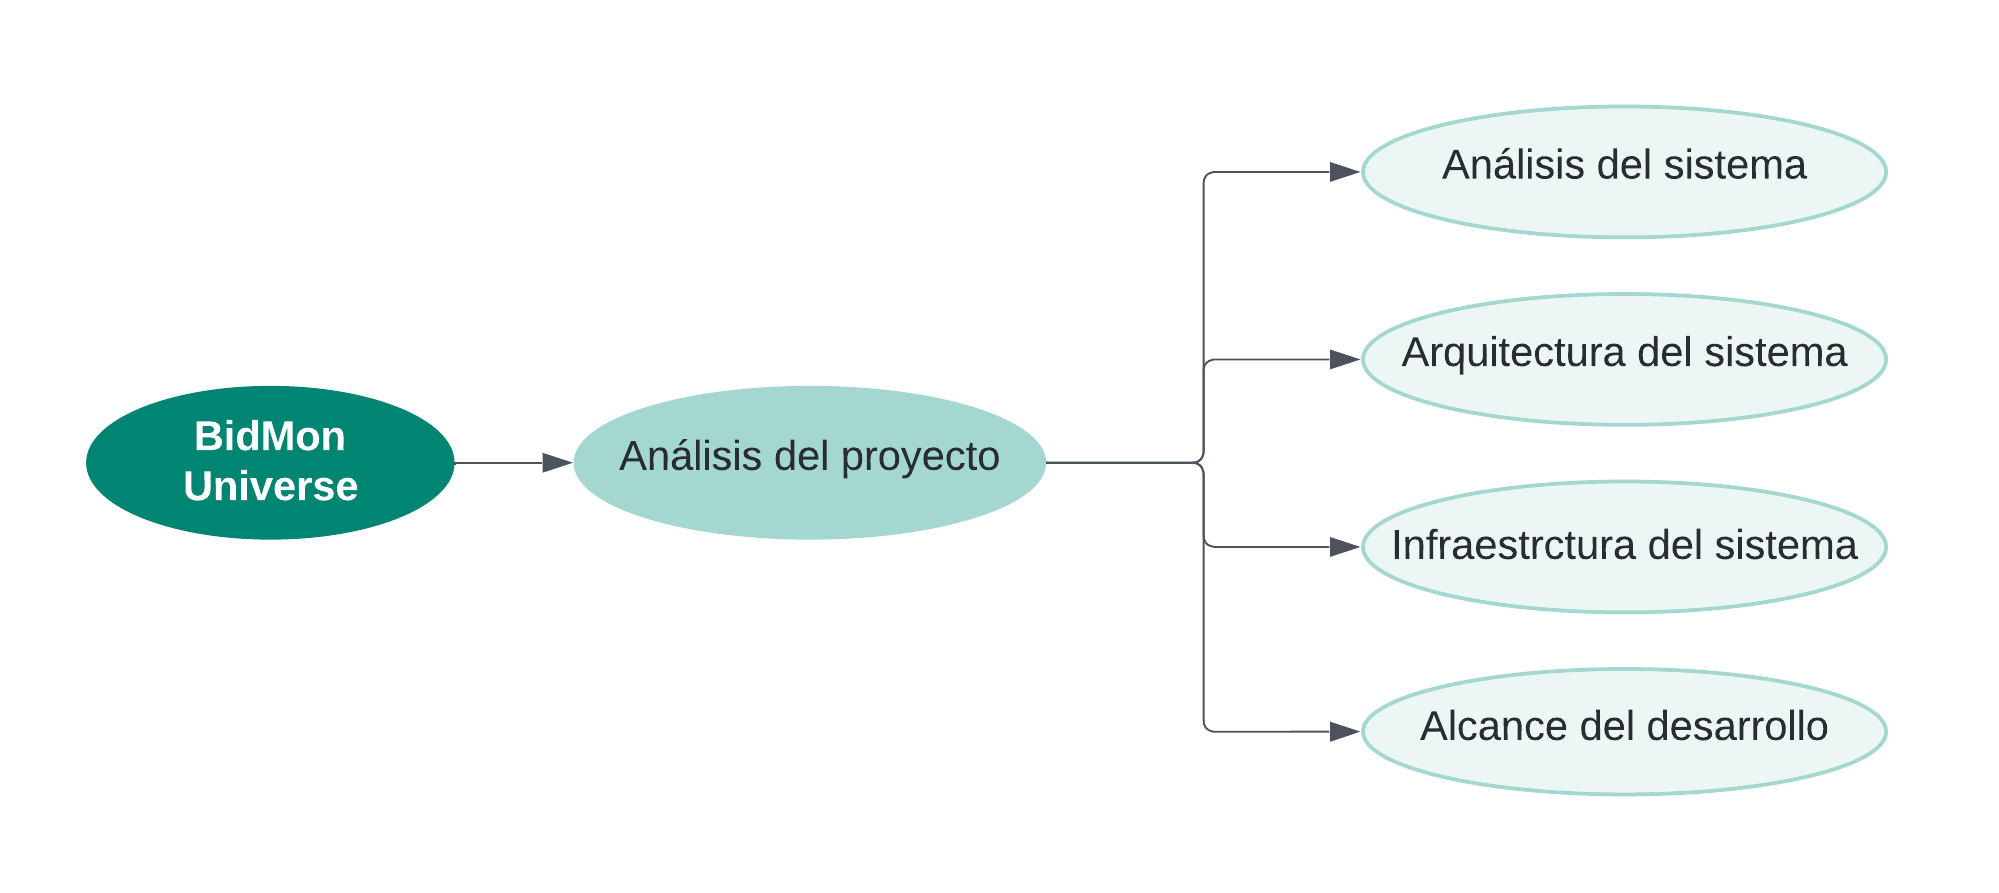
\includegraphics[width=0.7\linewidth]{figures/5-PBS/5_PBS-Analisis.png}
    \caption{PBS. Análisis del sistema}
    \label{fig:5_PBS-Analisis-Sistema}
\end{figure}

\subsubsection{PBS. Seguimiento del sistema}
En esta fase se detallan los productos que se obtienen en la fase de segumiento del proyecto, principalmente documentación e informes como se muestra en la \coloredUnderline{\hyperlink{fig:5_PBS-Seguimiento-Sistema}{Figura \ref*{fig:5_PBS-Seguimiento-Sistema}: \nameref*{fig:5_PBS-Seguimiento-Sistema}}}.
\begin{figure}[H]
    \hypertarget{fig:5_PBS-Seguimiento-Sistema}{}
    \centering
    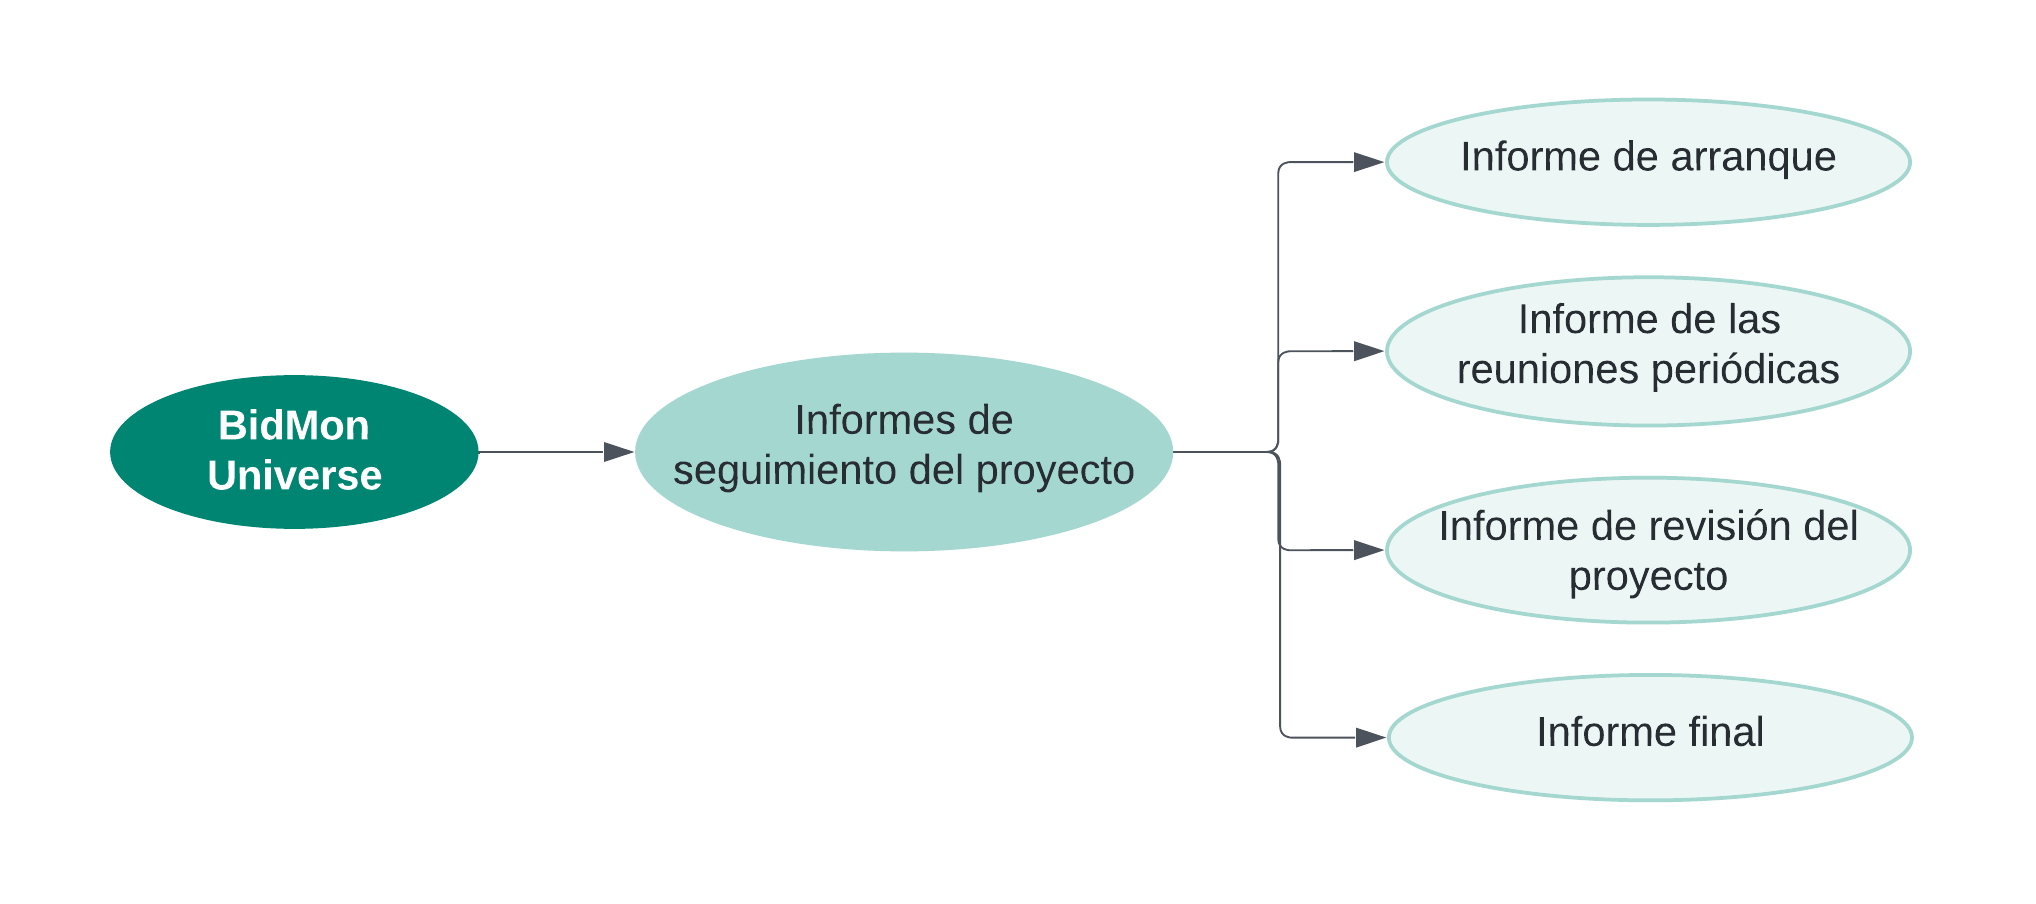
\includegraphics[width=0.7\linewidth]{figures/5-PBS/5_PBS-Seguimiento.png}
    \caption{PBS. Seguimiento del sistema}
    \label{fig:5_PBS-Seguimiento-Sistema}
\end{figure}

\subsubsection{PBS. Diseño del sistema}
En la \coloredUnderline{\hyperlink{fig:5_PBS-Diseño-Sistema}{Figura \ref*{fig:5_PBS-Diseño-Sistema}: \nameref*{fig:5_PBS-Diseño-Sistema}}}, se detallan los productos que se deben entregar en la fase de diseño del sistema.
\begin{figure}[H]
    \hypertarget{fig:5_PBS-Diseño-Sistema}{}
    \centering
    \includegraphics[width=0.9\linewidth]{figures/5-PBS/5_PBS-Diseno.png}
    \caption{PBS. Diseño del sistema}
    \label{fig:5_PBS-Diseño-Sistema}
\end{figure}

\subsubsection{PBS. Implementación del sistema}
En la \coloredUnderline{\hyperlink{fig:5_PBS-Implementación-Sistema}{Figura \ref*{fig:5_PBS-Implementación-Sistema}: \nameref*{fig:5_PBS-Implementación-Sistema}}}, se detallan los productos a realizar en la fase de implementación del sistema.
\begin{figure}[H]
    \hypertarget{fig:5_PBS-Implementación-Sistema}{}
    \centering
    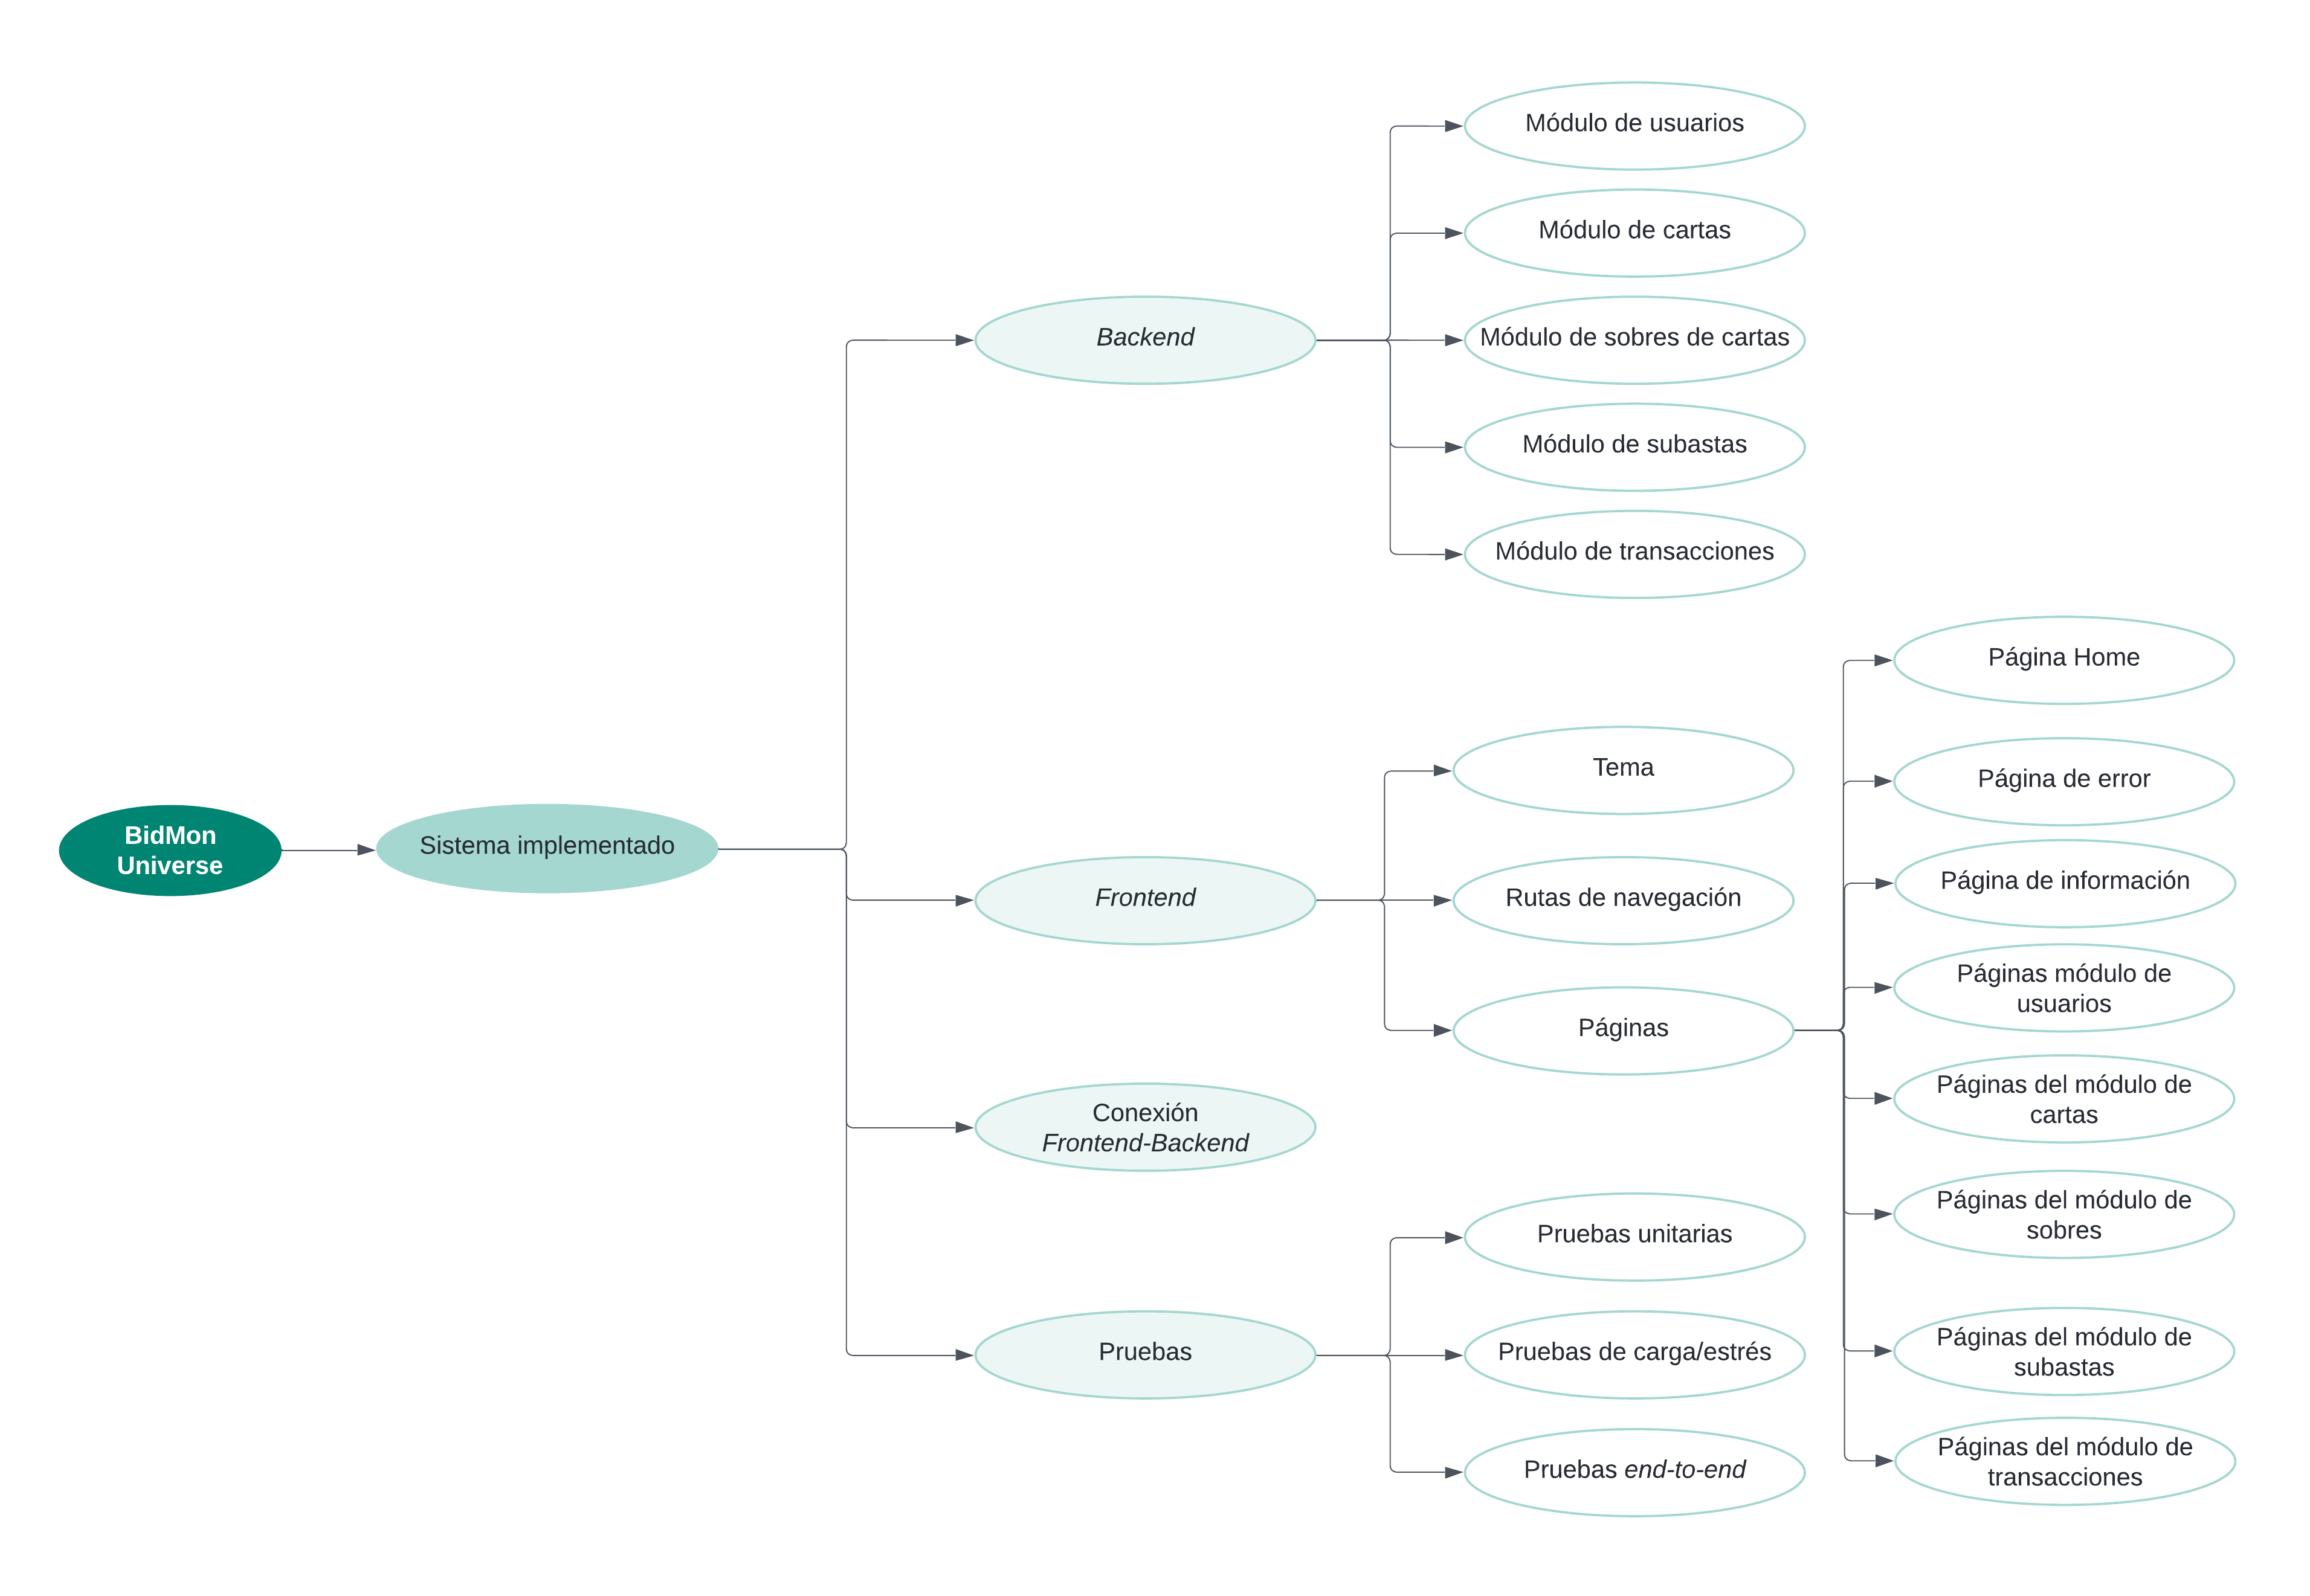
\includegraphics[width=0.9\linewidth]{figures/5-PBS/5_PBS-Implementacion.png}
    \caption{PBS. Implementación del sistema}
    \label{fig:5_PBS-Implementación-Sistema}
\end{figure}

\subsubsection{PBS. Pruebas del sistema}
En la fase de pruebas del sistema se obtienen como productos los resultados de la ejecución de dichas pruebas.
\begin{figure}[H]
    \hypertarget{fig:5_PBS-Pruebas-Sistema}{}
    \centering
    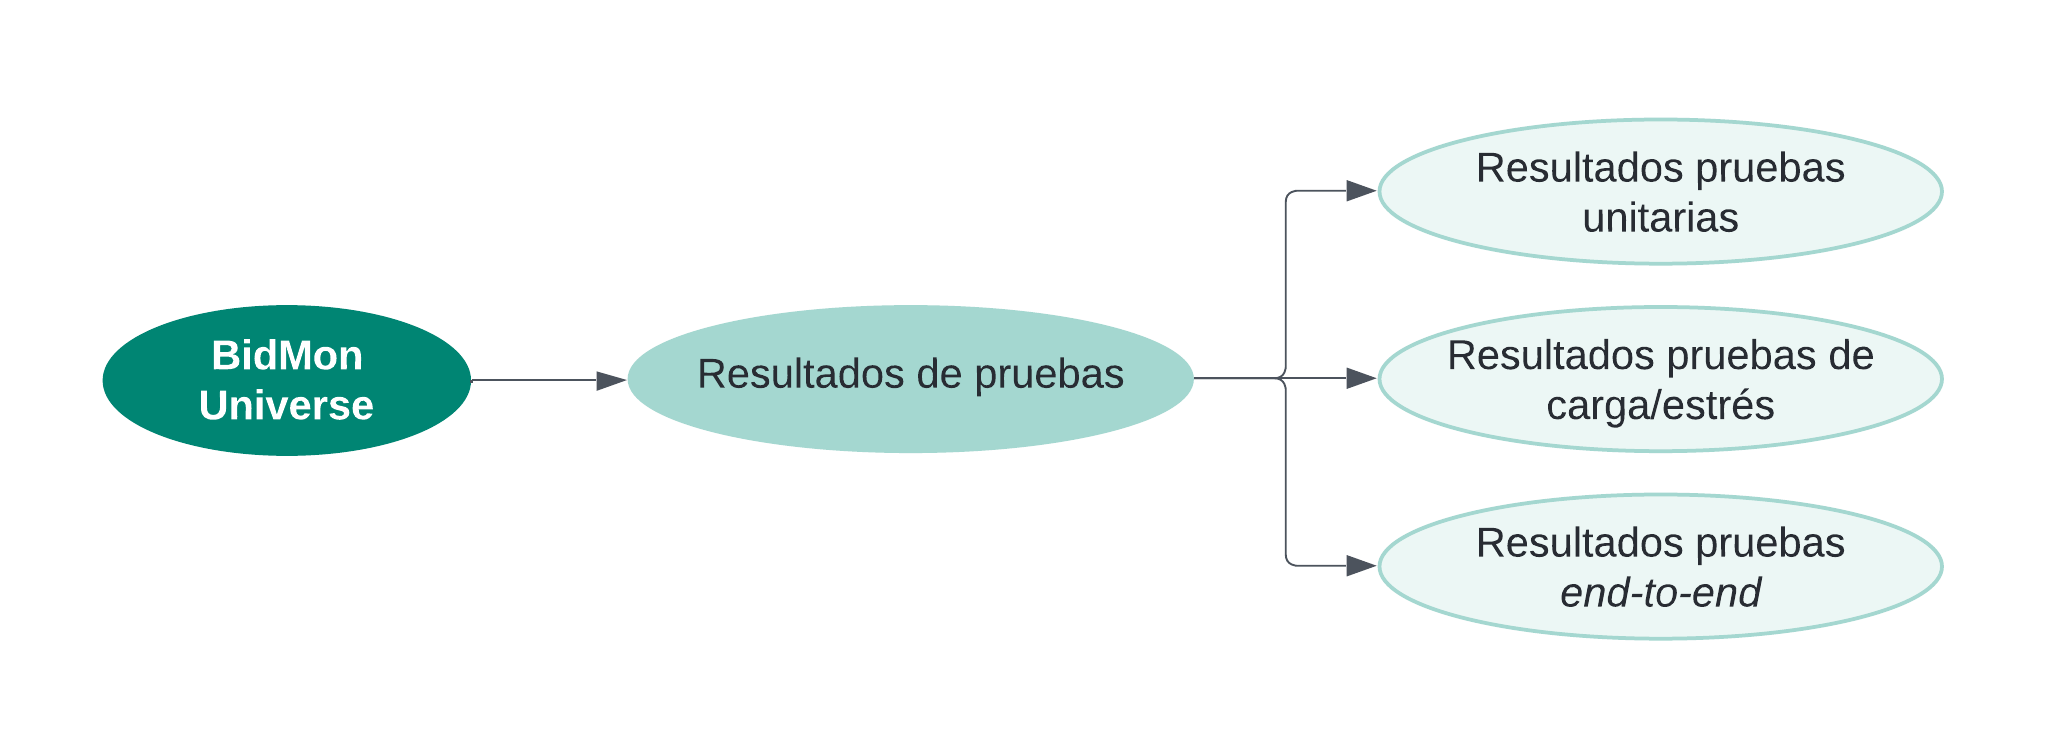
\includegraphics[width=0.7\linewidth]{figures/5-PBS/5_PBS-Pruebas.png}
    \caption{PBS. Pruebas del sistema}
    \label{fig:5_PBS-Pruebas-Sistema}
\end{figure}

\subsubsection{PBS. Despliegue del sistema}
En la fase de despliegue del sistema se obtiene como producto el sistema desplegado y en funcionamiento.
\begin{figure}[H]
    \hypertarget{fig:5_PBS-Despliegue-Sistema}{}
    \centering
    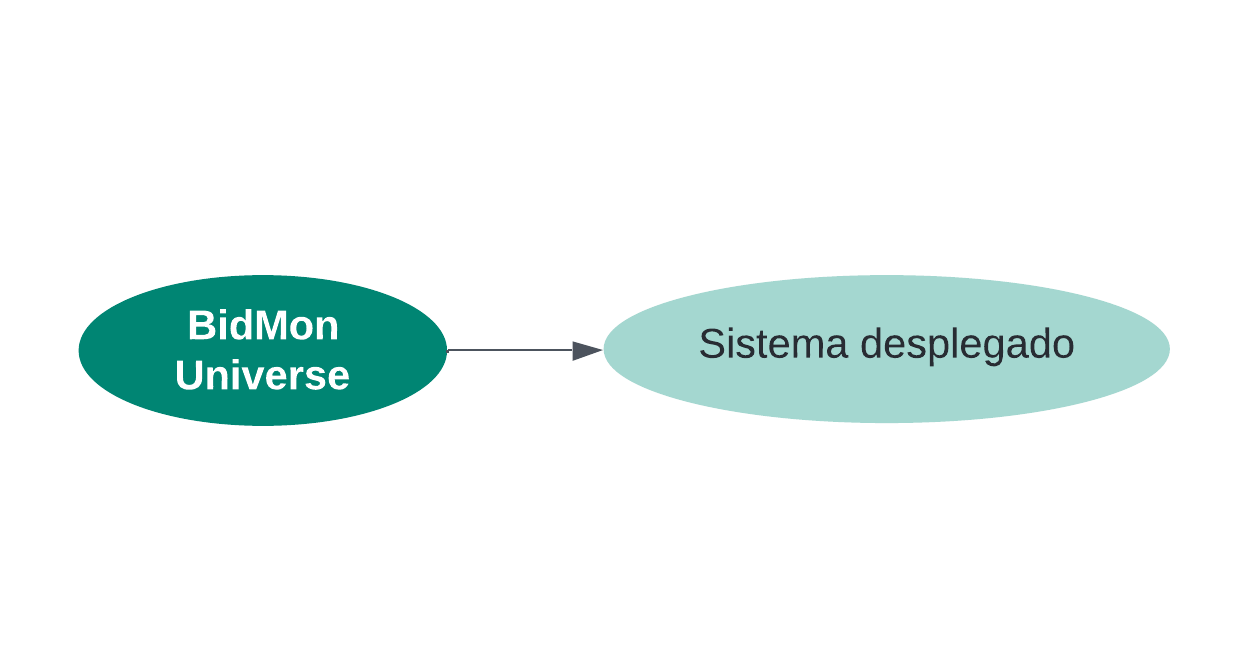
\includegraphics[width=0.7\linewidth]{figures/5-PBS/5_PBS-Despliegue.png}
    \caption{PBS. Despliegue del sistema}
    \label{fig:5_PBS-Despliegue-Sistema}
\end{figure}


\subsubsection{PBS. Documentación del sistema}
En la fase de documentación del sistema se obtienen como productos los documentos técnicos que describen el proyecto junto con los anexos.
\begin{figure}[H]
    \hypertarget{fig:5_PBS-Documentación-Sistema}{}
    \centering
    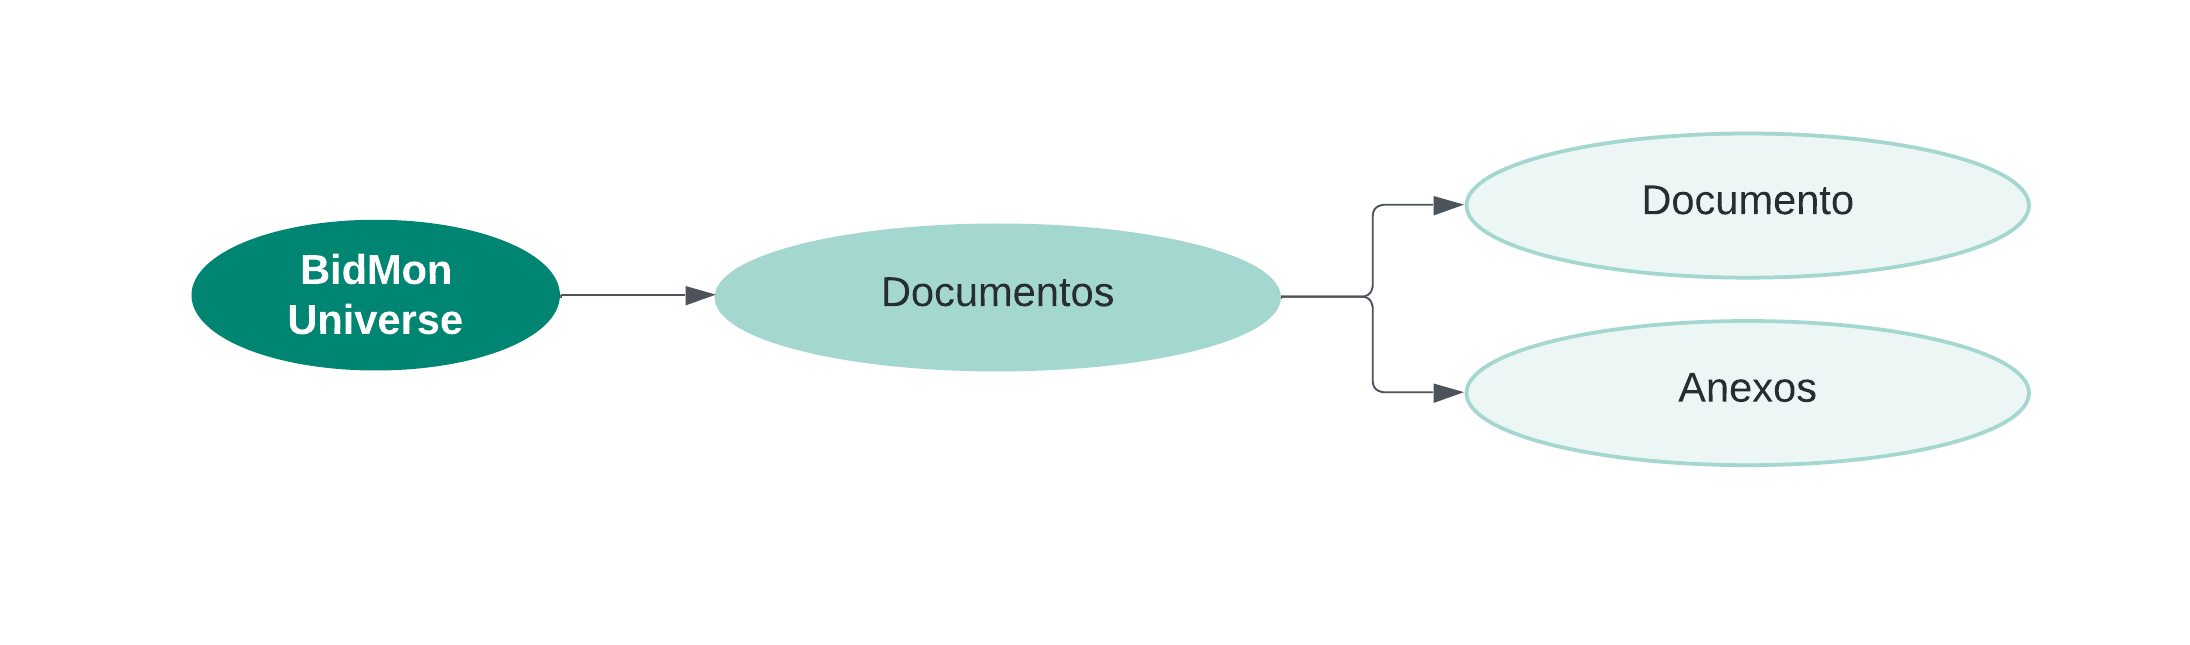
\includegraphics[width=0.7\linewidth]{figures/5-PBS/5_PBS-Documento.png}
    \caption{PBS. Documentación del sistema}
    \label{fig:5_PBS-Documentación-Sistema}
\end{figure}



\subsection{Planificación Inicial. WBS}
\subsubsection{WBS}
En esta sección se detalla la estructura de desglose del trabajo del proyecto también conocida como WBS, \textit{Work Breakdown Structure}. 
En ella se especifican las tareas necesarias para obtener los productos detallados en \coloredUnderline{\hyperlink{sec:5-PBS}{\ref*{sec:5-PBS} \nameref*{sec:5-PBS}}}.

Estas tareas se representan en forma de árbol jerárquico, donde cada rama representa una tarea y sus subramas las tareas que la componen.
El diagrama se ha dividido en las fases en las que se divide el proyecto para mejorar la legibilidad, facilitando la comprensión de las tareas y sub-tareas que se deben realizar en cada una de ellas.

\subsubsubsection{WBS. Visión general}
En la \coloredUnderline{\hyperlink{fig:5_WBS-Vision-General}{Figura \ref*{fig:5_WBS-Vision-General}: \nameref*{fig:5_WBS-Vision-General}}} se muestra la estructura de desglose del trabajo del proyecto de alto nivel, es decir, 
las tareas generales o fases que se deben realizar para cumplir con los objetivos del proyecto.
En las siguientes secciones, se entrará en detalle en cada una de las tareas.
\begin{figure}[H]
    \hypertarget{fig:5_WBS-Vision-General}{}
    \centering
    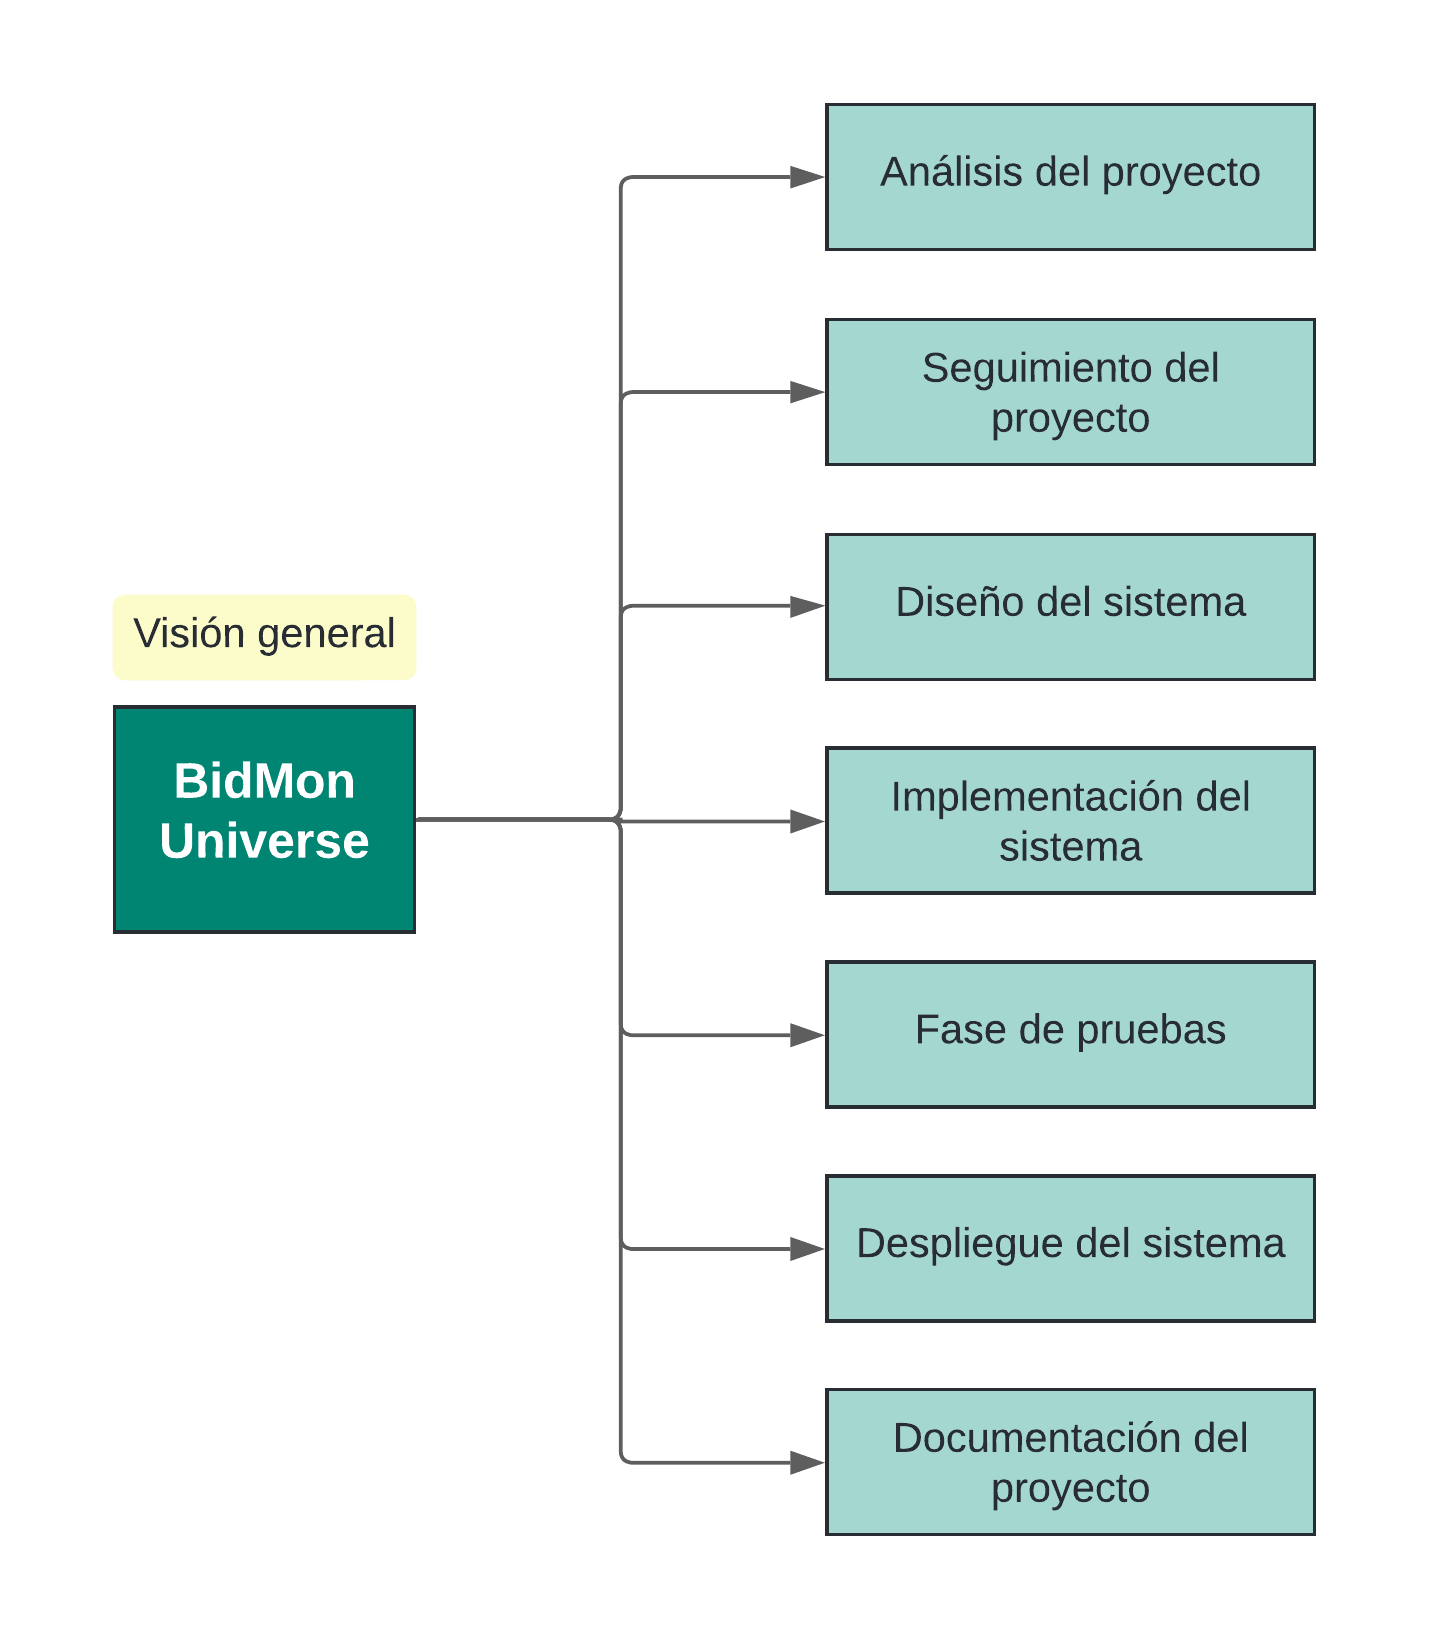
\includegraphics[width=0.5\linewidth]{figures/5-WBS/5_WBS-Vision-General.png}
    \caption{WBS. Visión general}
    \label{fig:5_WBS-Vision-General}
\end{figure}

\subsubsubsection{WBS. Análisis del proyecto}
En la \coloredUnderline{\hyperlink{fig:5_WBS-Analisis}{Figura \ref*{fig:5_WBS-Analisis}: \nameref*{fig:5_WBS-Analisis}}}, se detallan las tareas que se deben realizar en la fase de análisis del sistema para cumplir con los objetivos del proyecto.
\begin{figure}[H]
    \hypertarget{fig:5_WBS-Analisis}{}
    \centering
    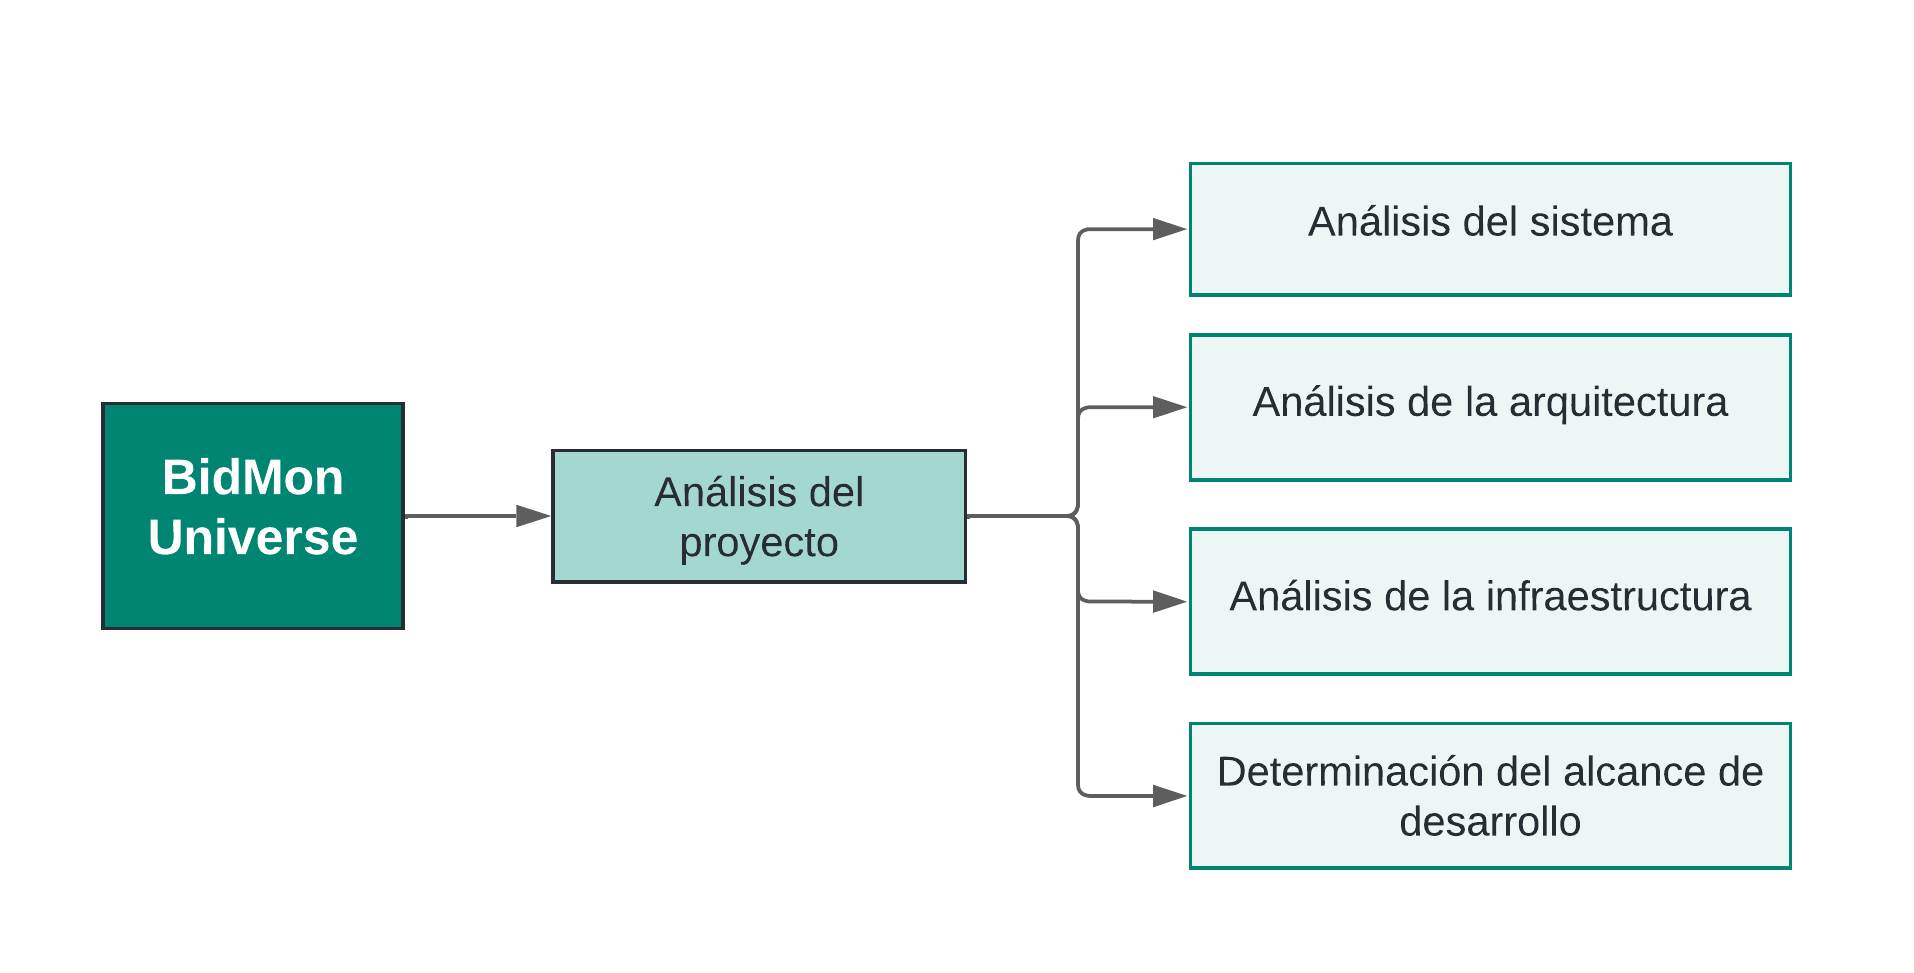
\includegraphics[width=0.7\linewidth]{figures/5-WBS/5_WBS-Analisis.png}
    \caption{WBS. Análisis del proyecto}
    \label{fig:5_WBS-Analisis}
\end{figure}

\subsubsubsection{WBS. Seguimiento del sistema}
En esta fase se realizan las tareas de seguimiento del proyecto, a través de distintas reuniones en las que se recopilará infomarción sobre el avance del proyecto. 
\begin{figure}[H]
    \hypertarget{fig:5_WBS-Seguimiento}{}
    \centering
    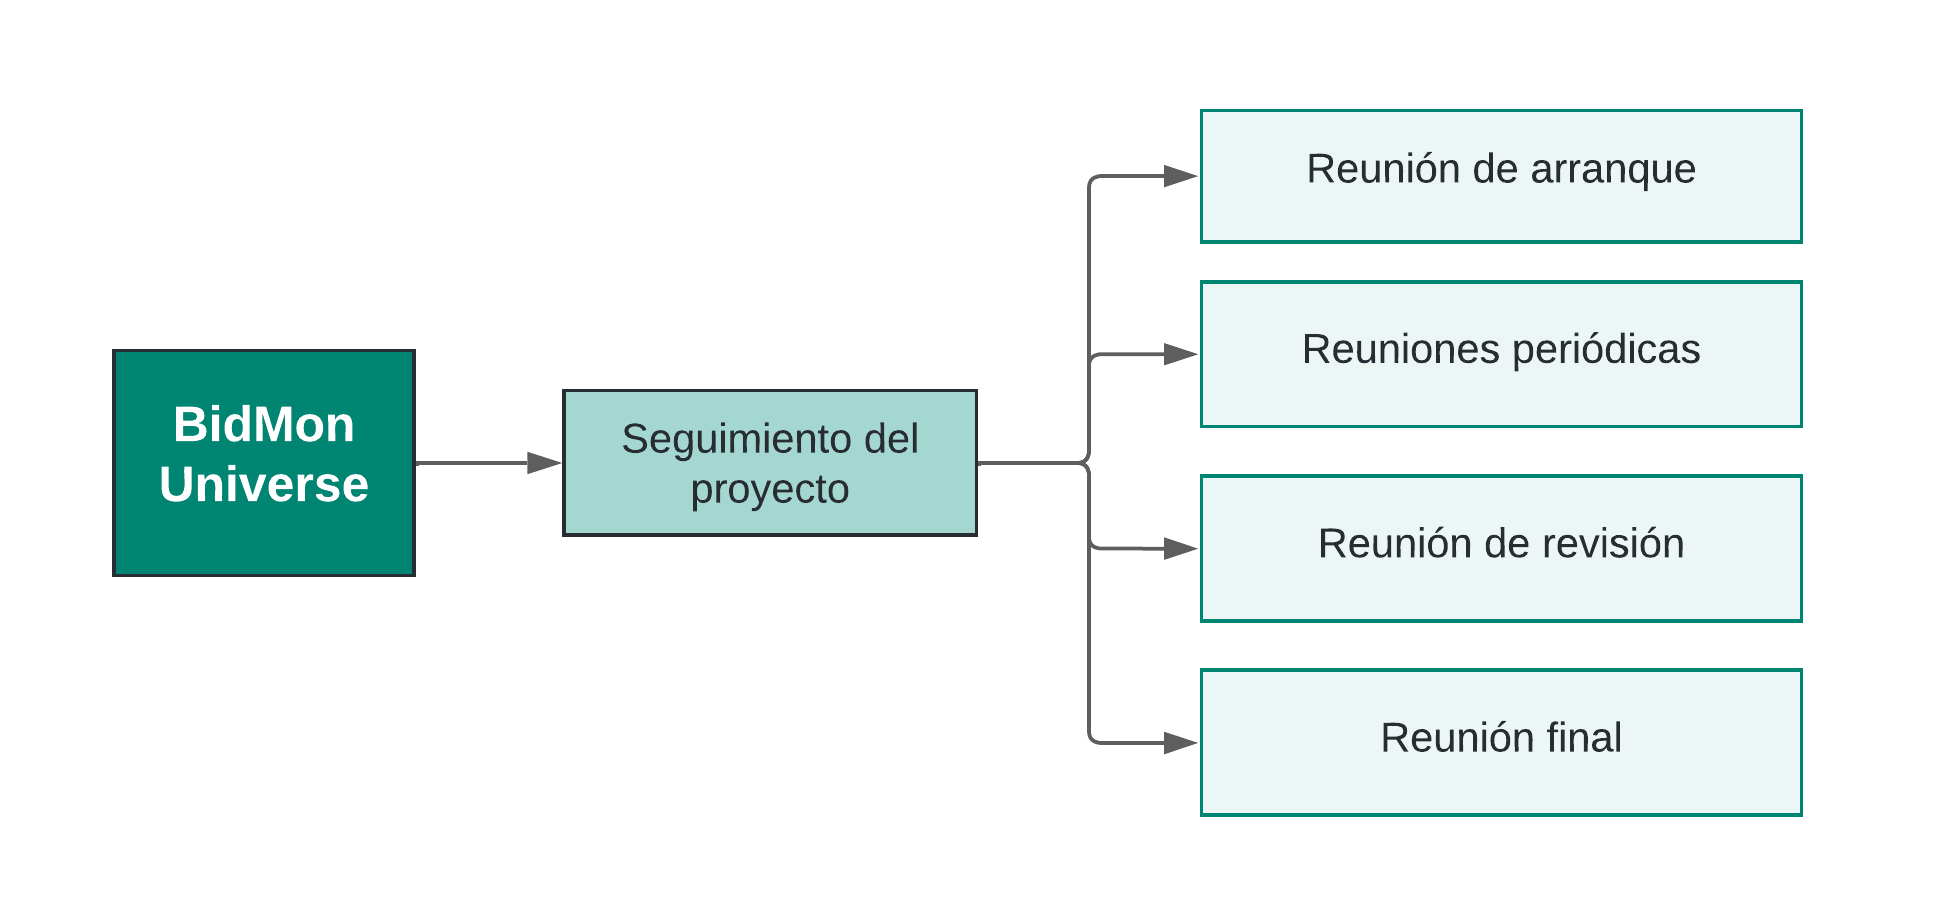
\includegraphics[width=0.7\linewidth]{figures/5-WBS/5_WBS-Seguimiento.png}
    \caption{WBS. Seguimiento del sistema}
    \label{fig:5_WBS-Seguimiento}
\end{figure}

\subsubsubsection{WBS. Diseño del sistema}
En la \coloredUnderline{\hyperlink{fig:5_WBS-Diseno}{Figura \ref*{fig:5_WBS-Diseno}: \nameref*{fig:5_WBS-Diseno}}}, se detallan las tareas que se deben realizar en la fase de diseño del sistema.
\begin{figure}[H]
    \hypertarget{fig:5_WBS-Diseno}{}
    \centering
    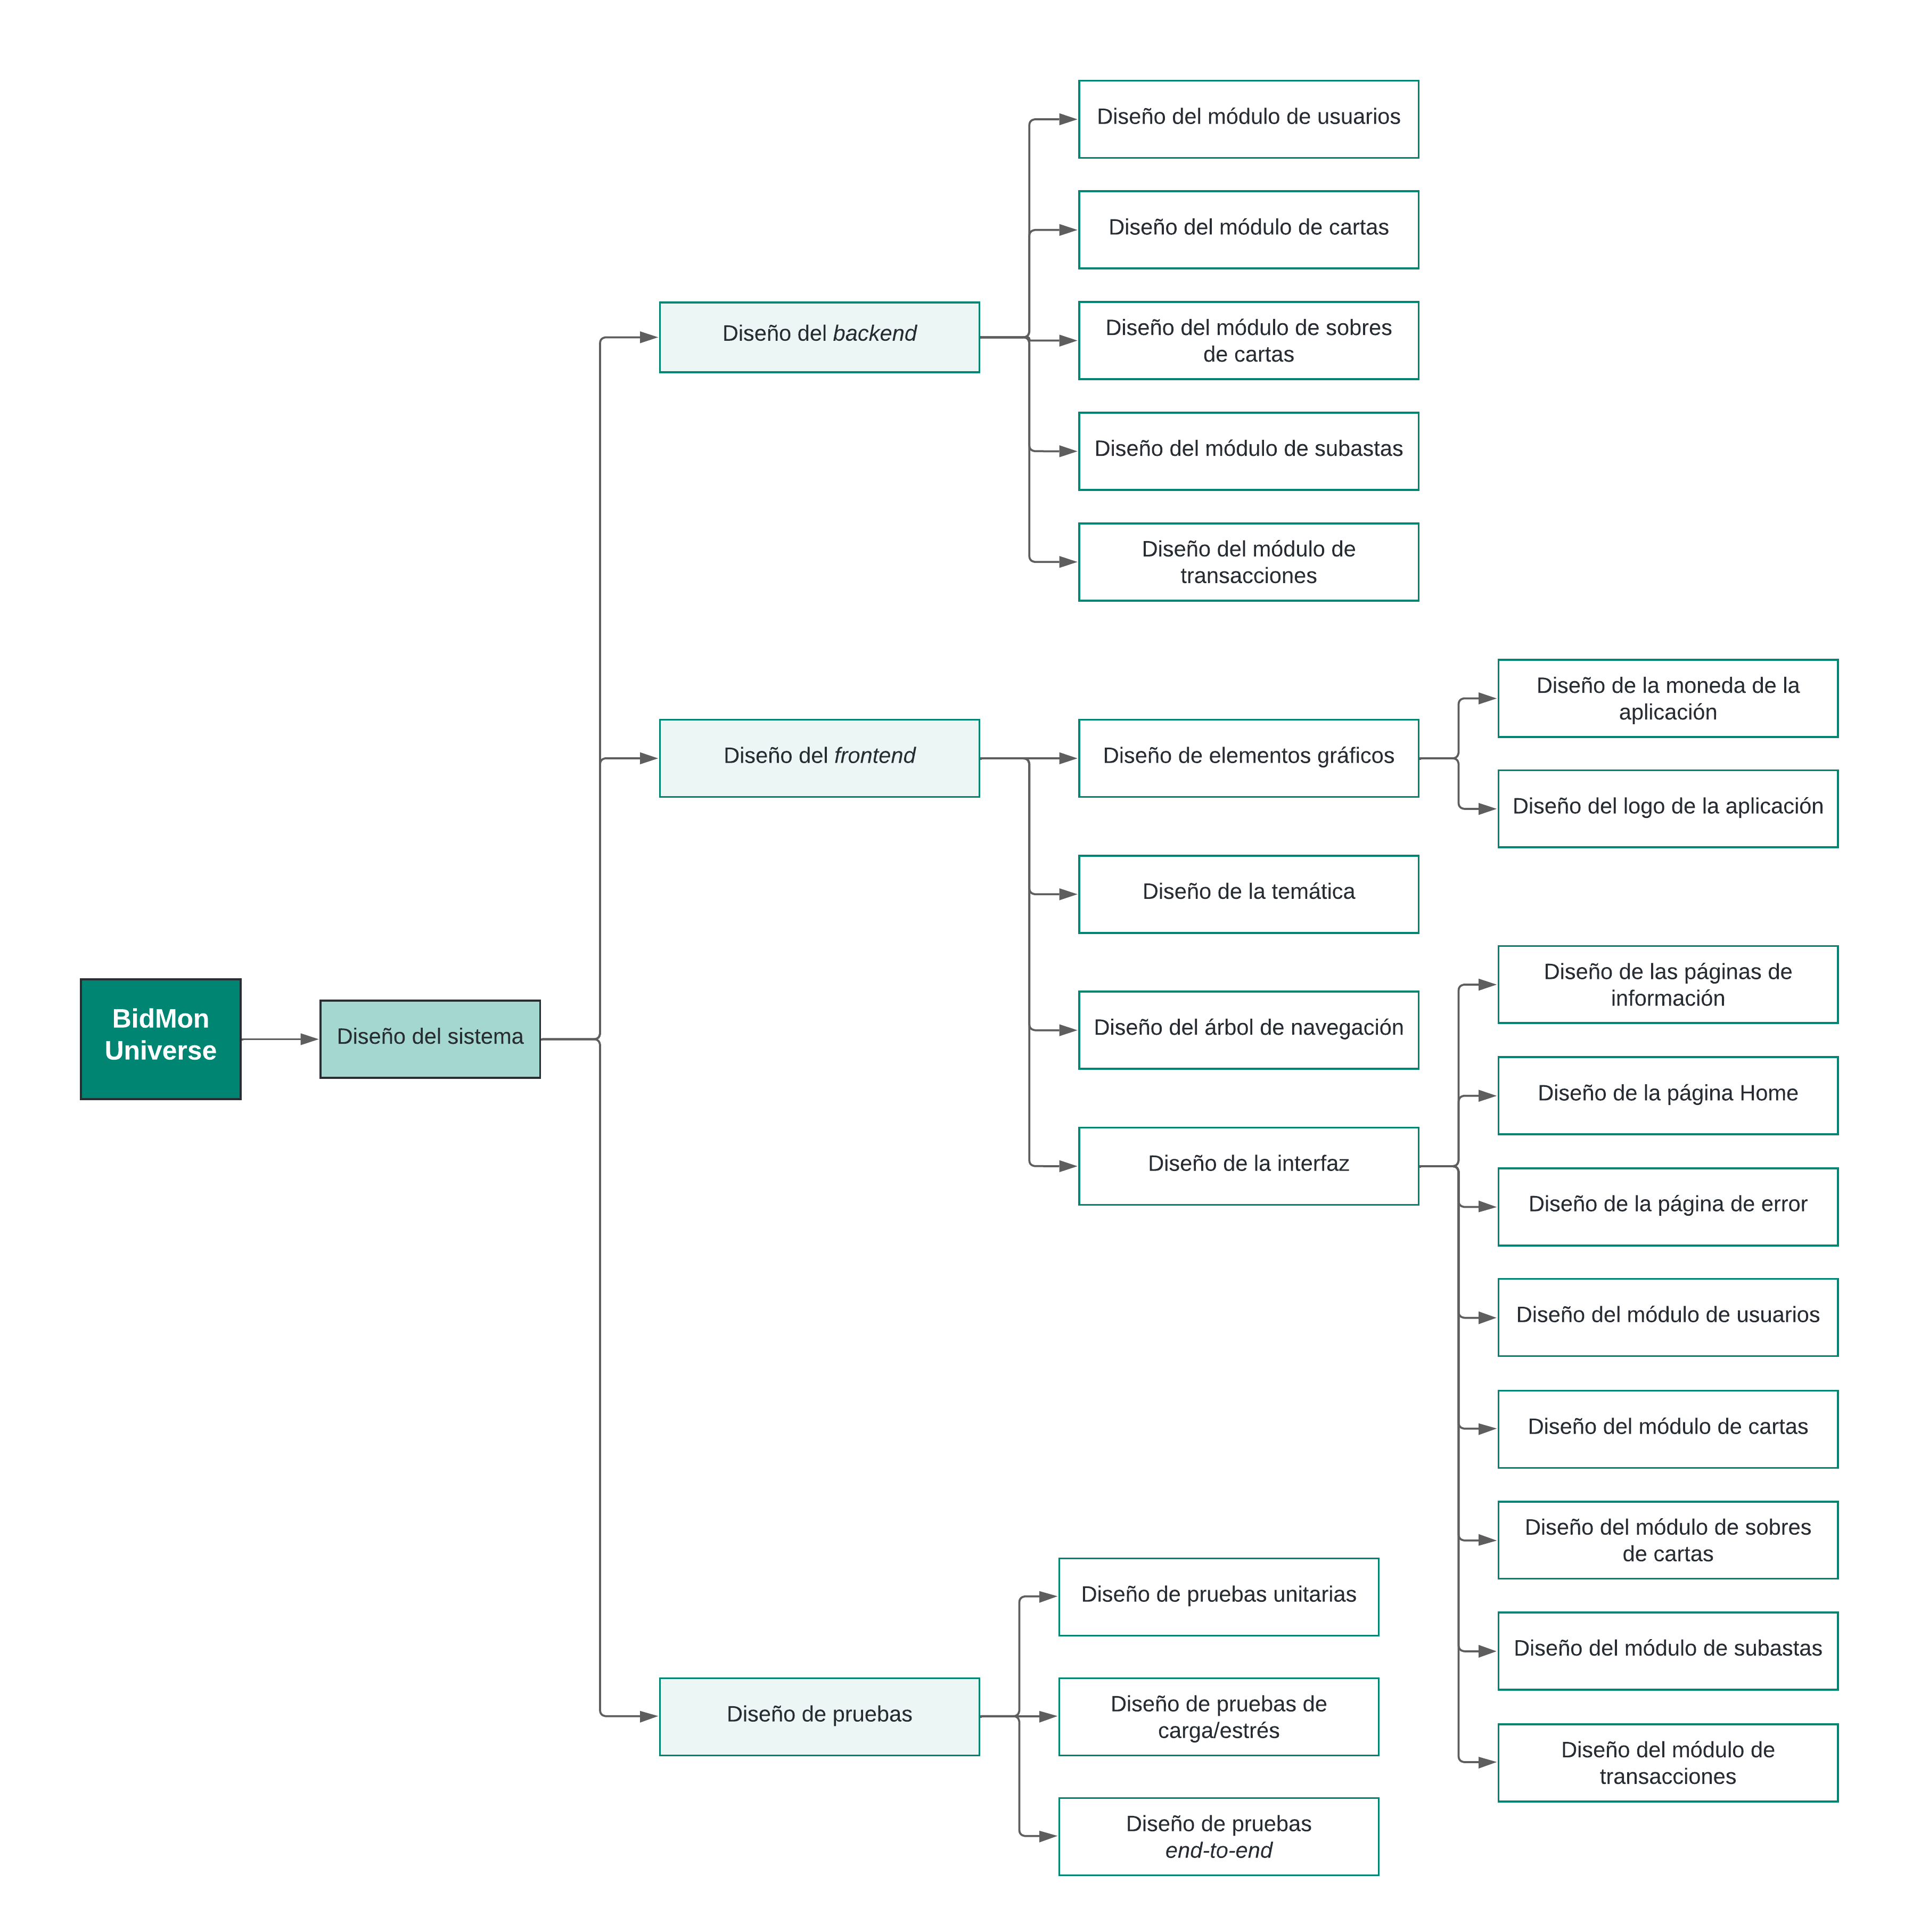
\includegraphics[width=0.9\linewidth]{figures/5-WBS/5_WBS-Diseno.png}
    \caption{WBS. Diseño del sistema}
    \label{fig:5_WBS-Diseno}
\end{figure}

\subsubsubsection{WBS. Implementación del sistema}
En la \coloredUnderline{\hyperlink{fig:5_WBS-Implementacion}{Figura \ref*{fig:5_WBS-Implementacion}: \nameref*{fig:5_WBS-Implementacion}}}, se detallan las tareas que se deben realizar en la fase de implementación del sistema.
\begin{figure}[H]
    \hypertarget{fig:5_WBS-Implementacion}{}
    \centering
    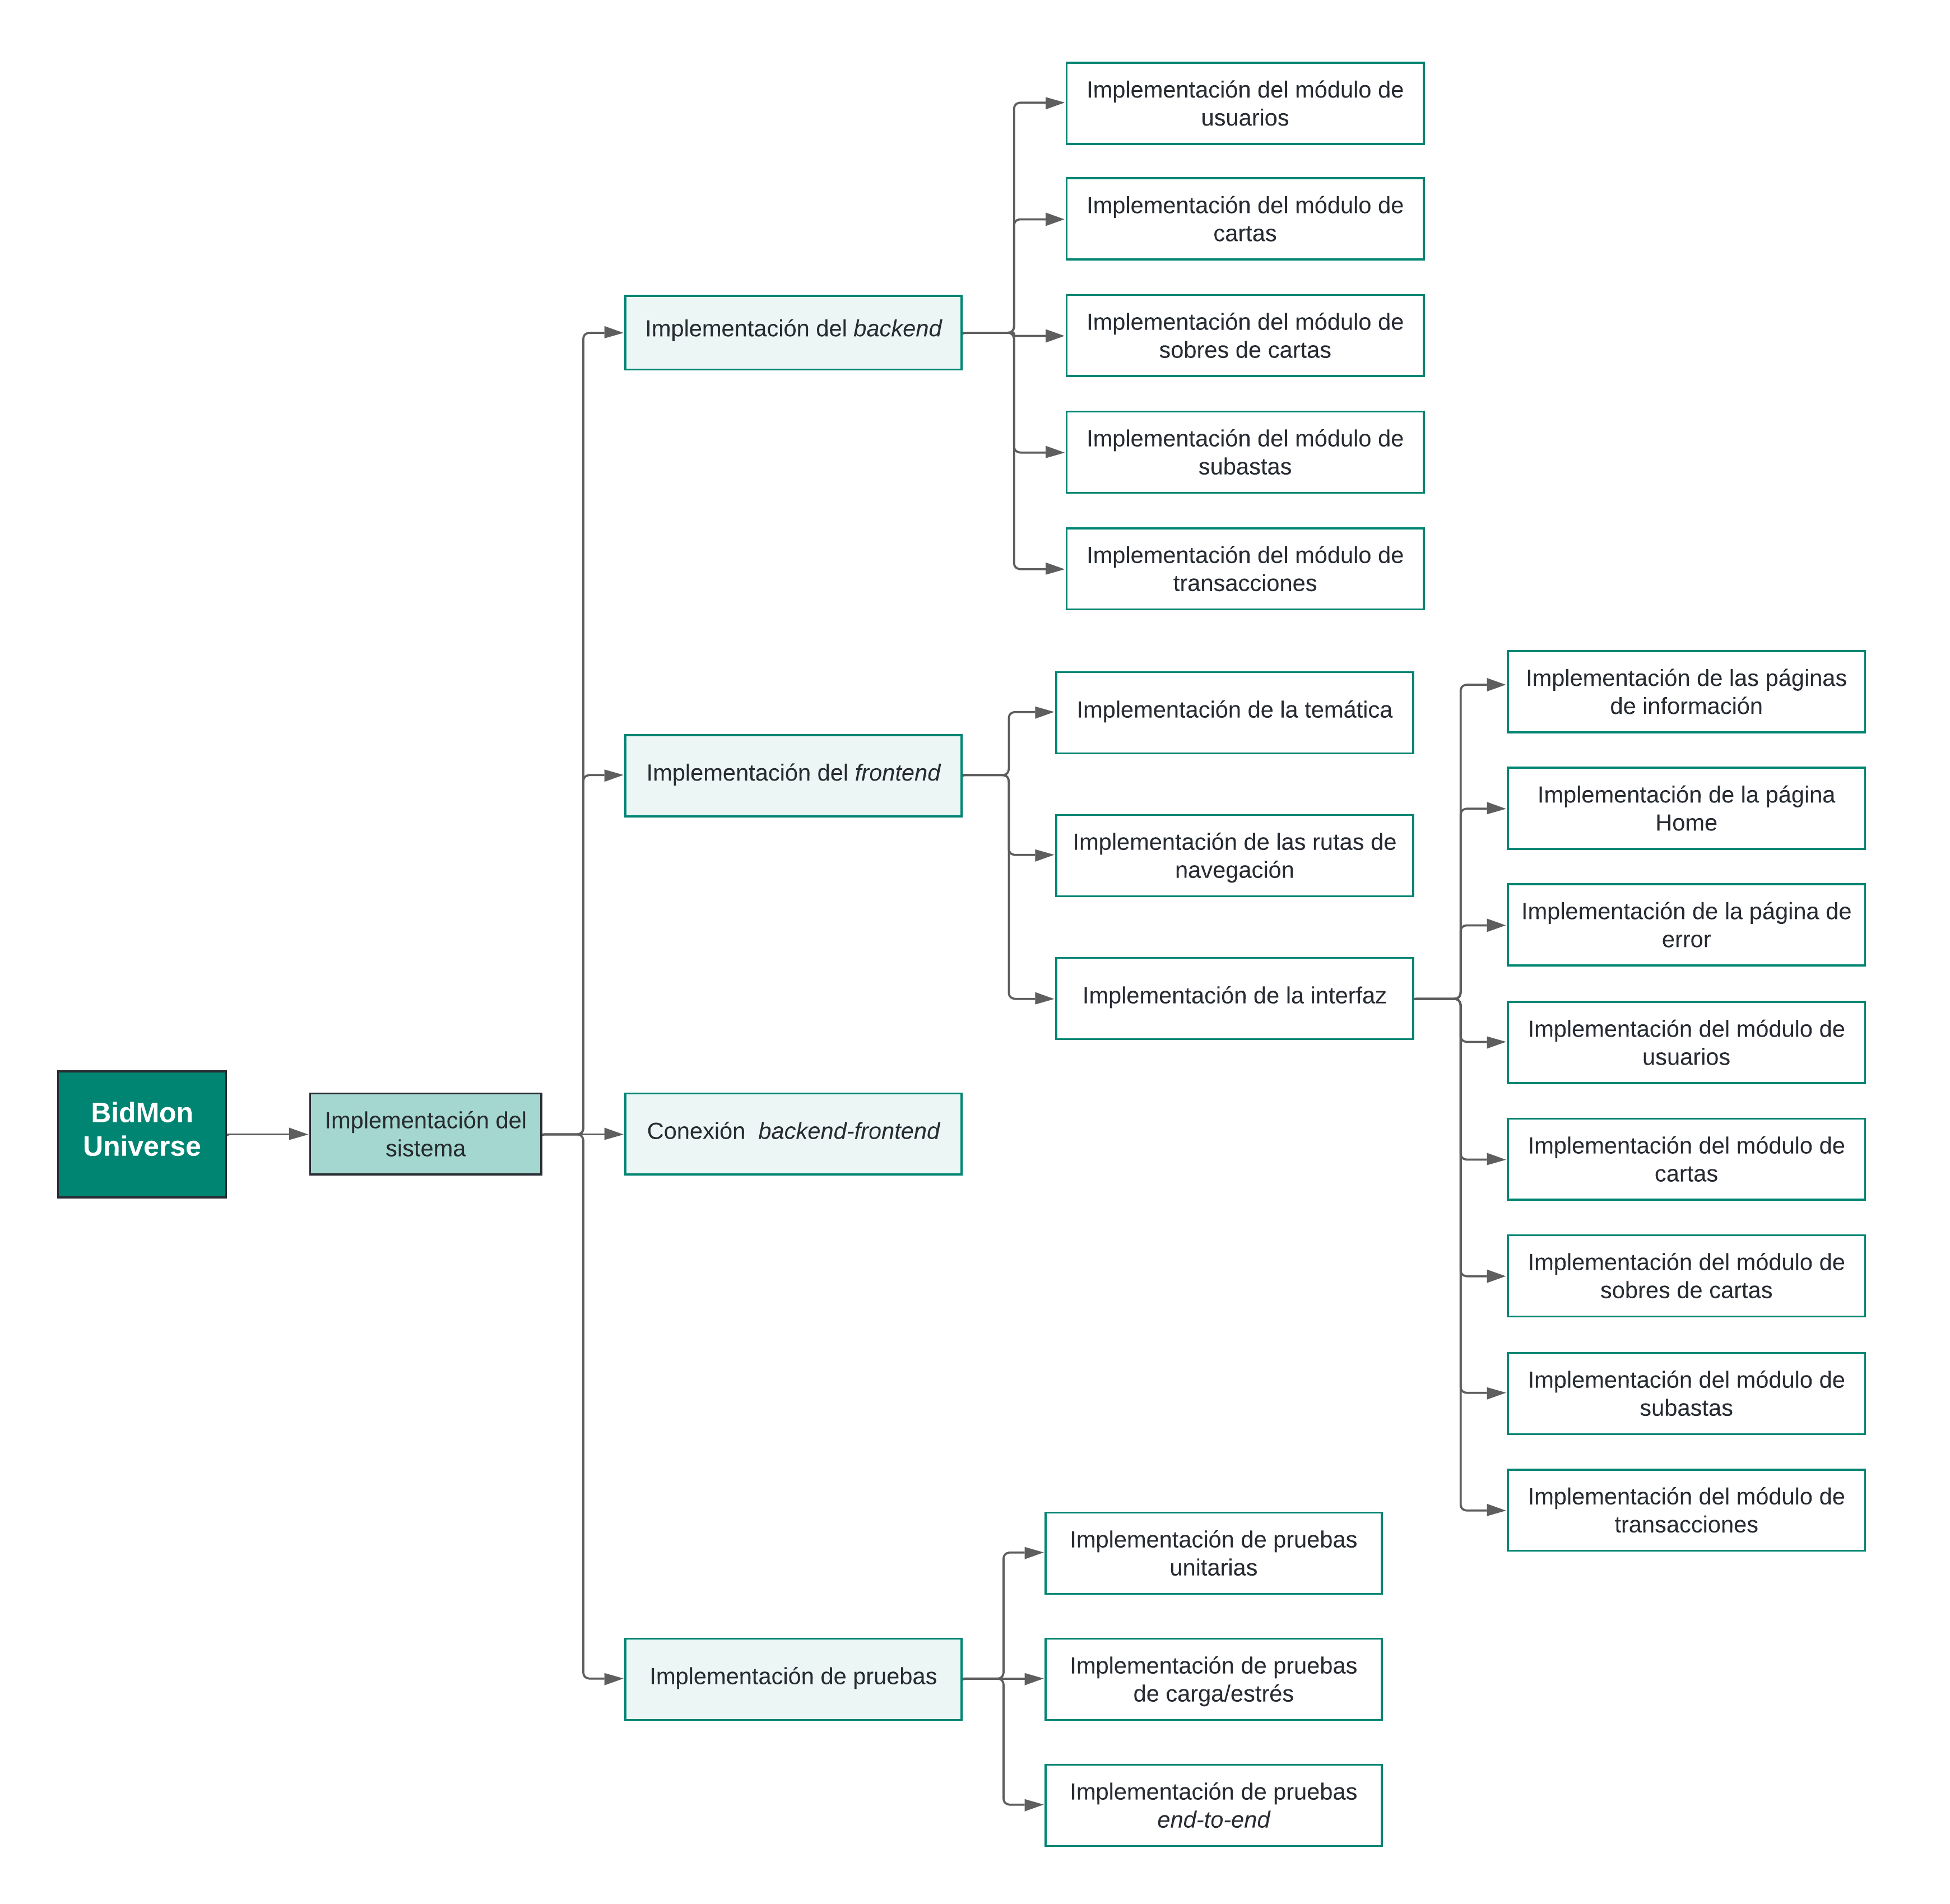
\includegraphics[width=0.9\linewidth]{figures/5-WBS/5_WBS-Implementacion.png}
    \caption{WBS. Implementación del sistema}
    \label{fig:5_WBS-Implementacion}
\end{figure}

\subsubsubsection{WBS. Fase de pruebas}
En la fase de pruebas del sistema se realizan las tareas necesarias para comprobar que el sistema cumple con los requisitos establecidos, recogiendo los informes especificados en \coloredUnderline{\hyperlink{fig:5_PBS-Pruebas}{Figura \ref*{fig:5_PBS-Pruebas}: \nameref*{fig:5_PBS-Pruebas}}}.
\begin{figure}[H]
    \hypertarget{fig:5_WBS-Pruebas}{}
    \centering
    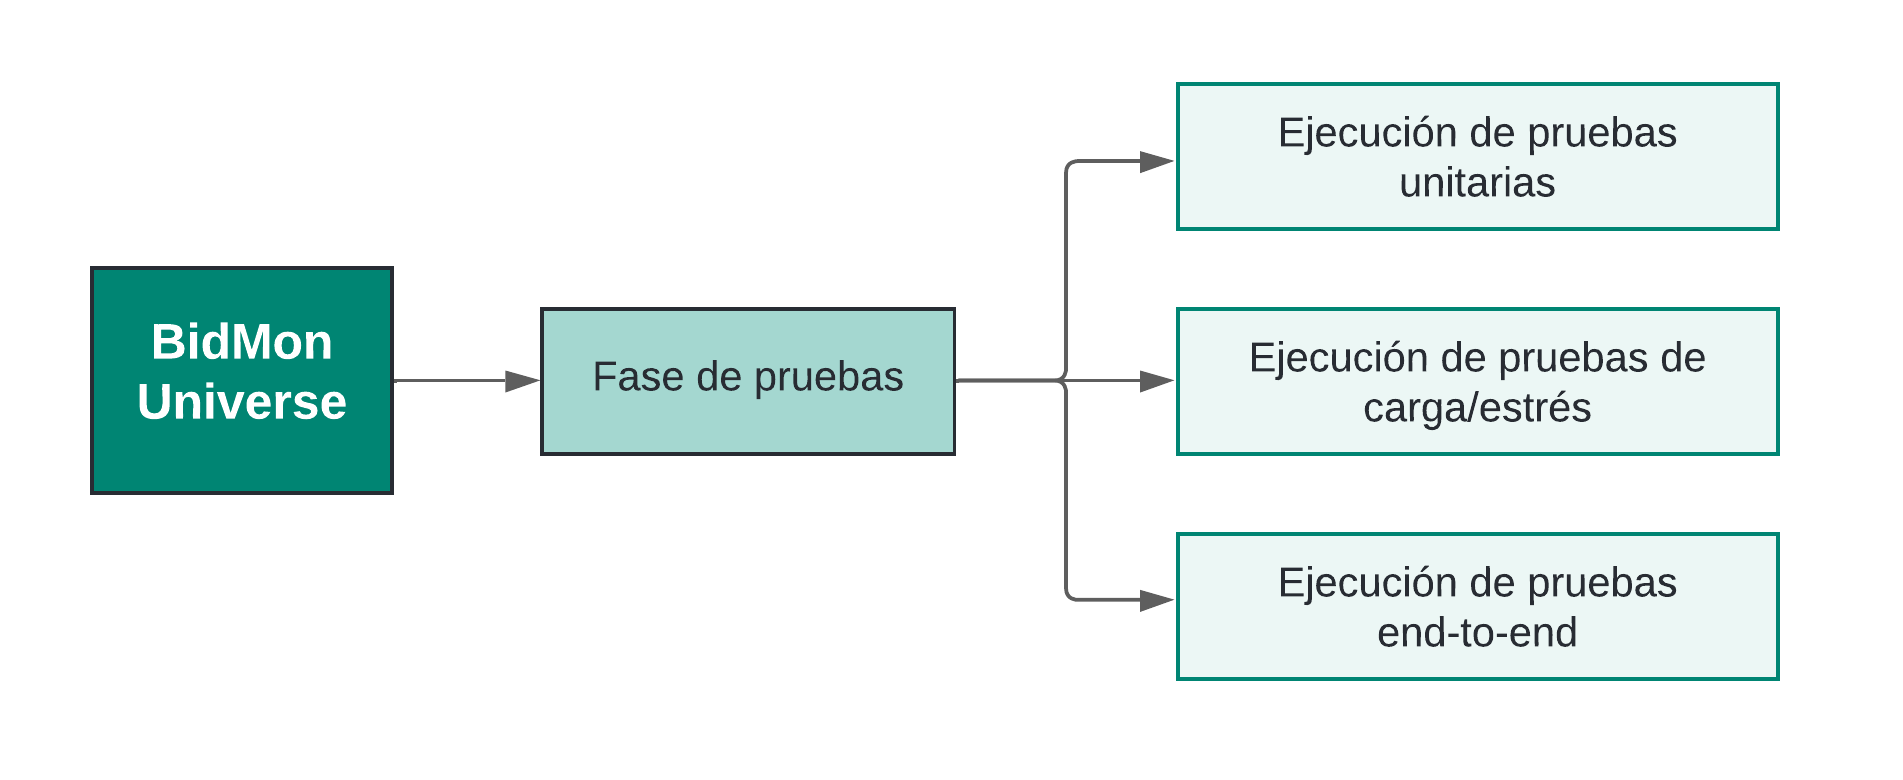
\includegraphics[width=0.9\linewidth]{figures/5-WBS/5_WBS-Pruebas.png}
    \caption{WBS. Fase de pruebas}
    \label{fig:5_WBS-Pruebas}
\end{figure}

\subsubsubsection{WBS. Despliegue del sistema}
En la fase de despliegue del sistema se realizan las tareas necesarias para poner en producción el sistema, como se detalla en la \coloredUnderline{\hyperlink{fig:5_WBS-Despliegue}{Figura \ref*{fig:5_WBS-Despliegue}: \nameref*{fig:5_WBS-Despliegue}}}.
\begin{figure}[H]
    \hypertarget{fig:5_WBS-Despliegue}{}
    \centering
    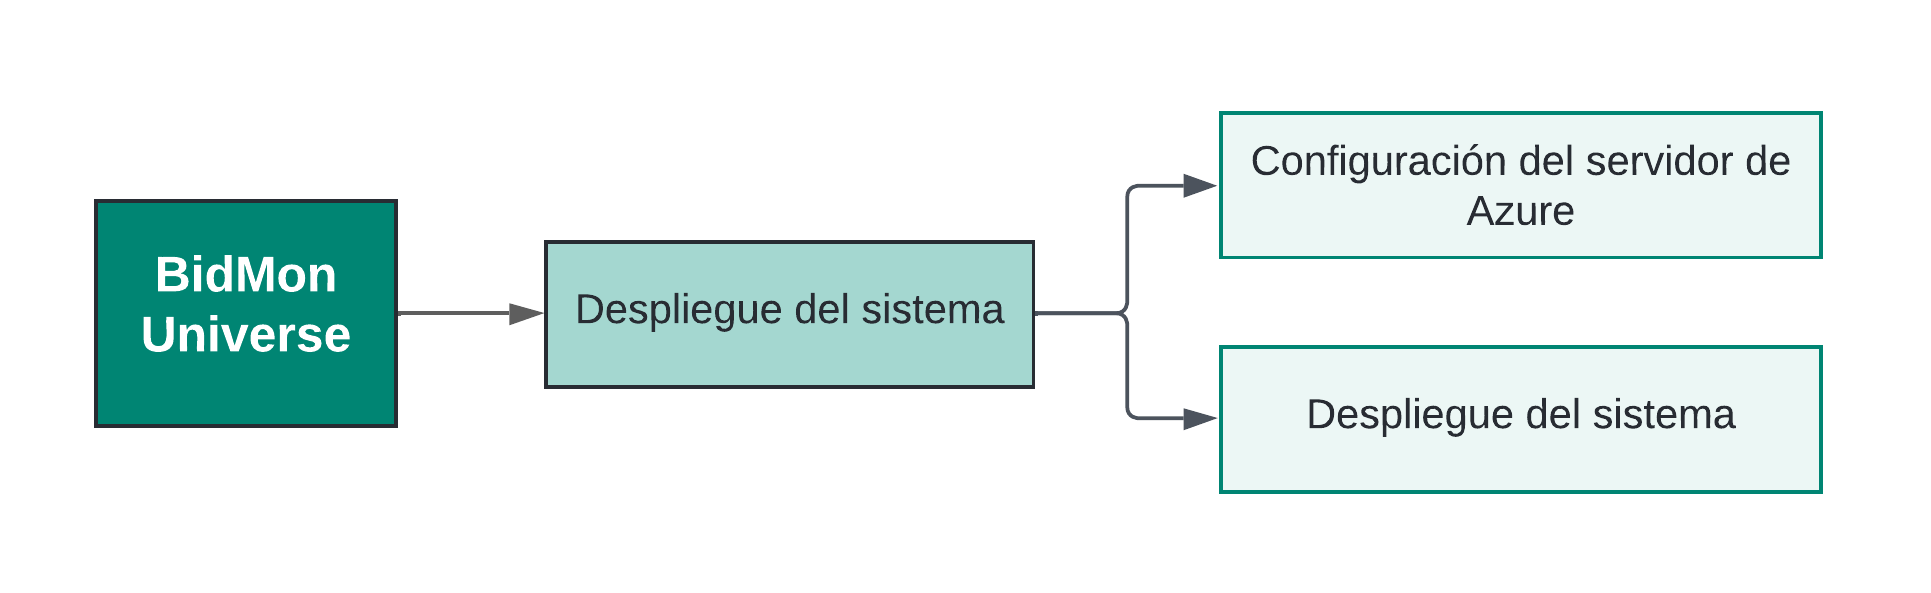
\includegraphics[width=0.9\linewidth]{figures/5-WBS/5_WBS-Despliegue2.png}
    \caption{WBS. Despliegue del sistema}
    \label{fig:5_WBS-Despliegue}
\end{figure}

\subsubsubsection{WBS. Documentación}
En la fase de documentación se realizan las tareas necesarias para la redacción de la memoria del proyecto, así como la preparación de la presentación del mismo.
\begin{figure}[H]
    \hypertarget{fig:5_WBS-Documentacion}{}
    \centering
    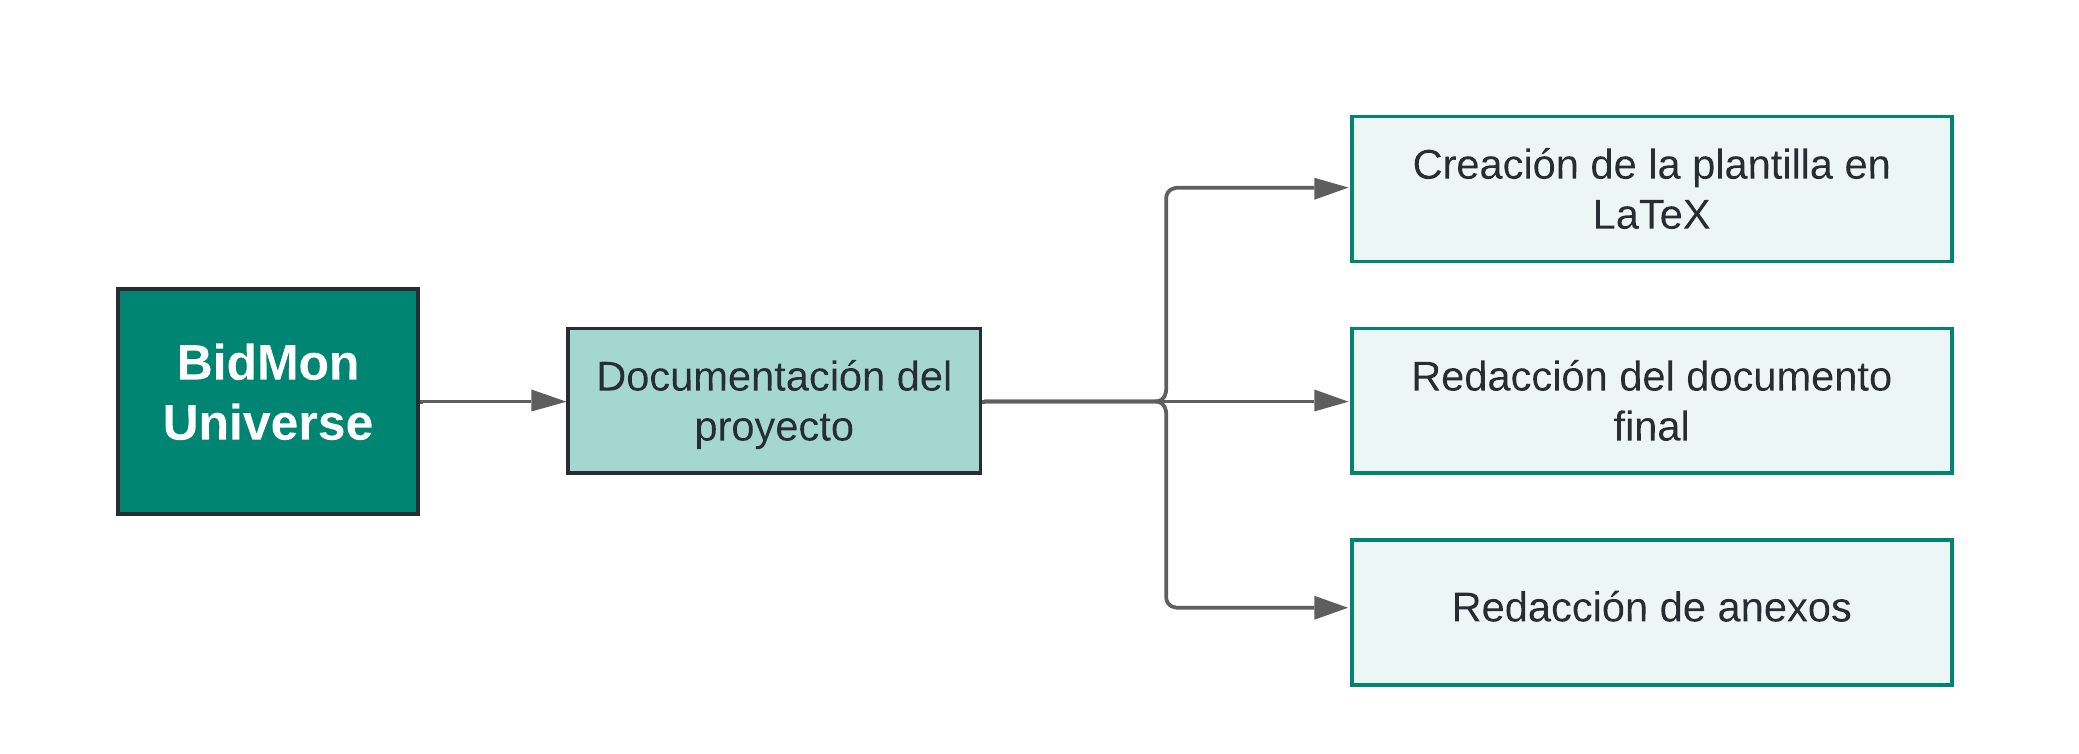
\includegraphics[width=0.9\linewidth]{figures/5-WBS/5_WBS-Documentacion.png}
    \caption{WBS. Documentación}
    \label{fig:5_WBS-Documentacion}
\end{figure}

\input{5-Planificacion-Gestion-TFG/5-Planificacion-inicial}


\subsection{Riesgos}
\subsubsection{Plan de Gestión de Riesgos} 

\subsubsection{Identificación de Riesgos}


\subsubsection{Registro de Riesgos} 

\begin{table}[htb]
    \centering
    \caption{Análisis de riesgo}
    \label{table:risk_analysis}
    \begin{tabular}{>{\columncolor{rowcolor}}l l l}
    \toprule
    \rowcolor{lightgreen}
    \textbf{Identificador} & \multicolumn{2}{l}{1} \\
    \midrule
    \textbf{Nombre} & \multicolumn{2}{l}{Problema de costos} \\
    \midrule
    \textbf{Descripción} & \multicolumn{2}{p{10cm}}{El costo de desarrollar y mantener un sitio web y un sistema de venta y distribución es alto, lo que puede afectar negativamente la rentabilidad de la empresa si no se generan suficientes ingresos para cubrir estos costos.} \\
    \midrule
    \textbf{Categoría} & \multicolumn{2}{l}{Riesgo de gestión} \\
    \midrule
    \textbf{Probabilidad} & \multicolumn{2}{l}{Media} \\
    \midrule
    \textbf{Impacto} & Presupuesto & Crítico \\
    \cmidrule(lr){2-3}
    & Planificación & Medio \\
    \cmidrule(lr){2-3}
    & Alcance & Alto \\
    \cmidrule(lr){2-3}
    & Calidad & Alto \\
    \cmidrule(lr){2-3}
    & Total & 0.45 \\
    \midrule
    \textbf{Respuesta} & \multicolumn{2}{p{10cm}}{Realizar un análisis financiero riguroso para determinar el costo total del proyecto, incluyendo los costos de desarrollo, mantenimiento, actualizaciones y otros gastos asociados. Establecer proyecciones financieras realistas para garantizar que la empresa pueda generar suficientes ingresos para cubrir estos costos y obtener una rentabilidad adecuada.} \\
    \midrule
    \textbf{Estrategia} & \multicolumn{2}{l}{Mitigar el riesgo} \\
    \bottomrule
    \end{tabular}
    \end{table}





\subsection{Presupuesto Inicial}

\subsubsection{Presupuesto de Costes}

\subsubsection{Presupuesto de Cliente} 


\newpage
\section{EJECUCIÓN DEL PROYECTO}
\subsection{Plan Seguimiento de Planificación}
El criterio de seguimiento de la planificación se basará en la comparación de las tareas planificadas con las tareas realizadas, 
para ello se usará la planificación inicial como referencia. 
Se llevará a cabo un seguimiento semanal de las tareas realizadas, ayudándose de herramientas como Trello
\coloredUnderline{\href{https://trello.com/}{Trello}} y GitHub.

Si se detecta que una tarea no se ha completado en el tiempo estimado, se analizarán las causas y se reevaluará la planificación para ajustar los plazos 
y recursos necesarios. Estas desviaciones se registrarán en la bitácora de incidencias del proyecto.

En el caso de que se detecten desviaciones significativas en la planificación, se informará al jefe del proyecto y se tomarán las medidas necesarias 
para corregir la situación.

\subsection{Bitácora de Incidencias del Proyecto}

A lo largo del proyecto se han registrado las siguientes incidencias:
\begin{longtable}{
    >{\columncolor{lightgreen!20}}p{8cm}
    p{4cm}
    p{4cm}
    }
    \caption{Bitácora de incidencias del proyecto} \label{table:registro-incidencias} \\
    \toprule
    \rowcolor{darkgreen!50}
    \textbf{Descripción} & \multicolumn{1}{>{\columncolor{darkgreen!50}\centering\arraybackslash}p{4cm}}{\textbf{Solución}} & \multicolumn{1}{>{\columncolor{darkgreen!50}\centering\arraybackslash}p{4cm}}{\textbf{Efecto en la planificación}} \\
    \endfirsthead
    
    \multicolumn{3}{c}%
    {{ \tablename\ \thetable{} Bitácora de incidencias del proyecto -- continuación de la página anterior}} \\
    \toprule
    \rowcolor{darkgreen!50}
    \textbf{Descripción} & \multicolumn{1}{>{\columncolor{darkgreen!50}\centering\arraybackslash}p{4cm}}{\textbf{Solución}} & \multicolumn{1}{>{\columncolor{darkgreen!50}\centering\arraybackslash}p{4cm}}{\textbf{Efecto en la planificación}} \\
    \midrule
    \endhead
    
    \midrule
    \multicolumn{3}{r}{{Continúa en la siguiente página...}} \\ 
    \endfoot
    
    \bottomrule
    \endlastfoot
    
    \midrule
    \textbf{Falta de análisis del sistema antes de realizar la planificación }. & Reunión de equipo para acordar el alcance del sistema y revisión de la planificación & Aumento del tiempo dedicado a la realización de la planificación \\
    \midrule
    \textbf{Desviación en la estimación de tiempo de diseño del modelo de datos} & Reunión de equipo para reevaluar la estrategia de diseño & Aumento del tiempo dedicado al diseño del sistema \\
    \midrule
    \textbf{Problemas de compatibilidad horaria del equipo de desarrollo con su trabajo actual} & Reducción del calendario del recurso & Aumento de los plazos de entrega \\
    \midrule
    \textbf{Nuevos requisitos no contemplados en la planificación inicial} & Corrección de la planificación y actualización de los requisitos y alcance del sistema. & Aumento de los plazos de entrega \\
    \midrule
    \textbf{Desviación en la estimación de tiempo de despliegue de la plataforma} & Configurar el sistema para que pueda comunicarse mediante el protocolo HTTPS & Aumento del tiempo dedicado al despliegue de la plataforma \\
    \midrule
    \textbf{Rehacer documento final de la memoria} & Se han adaptado los apartados del documento acorde a la plataforma que se está desarrollando & Aumento del tiempo dedicado a la redacción de la memoria \\
    \bottomrule
\end{longtable}

\subsection{Riesgos}
De los riesgos identificados en la planificación inicial, \coloredUnderline{\hyperlink{anexo:registro_de_riesgos}{Registro de riesgos}}, se han producido los siguientes:
\begin{itemize}
    \item \textbf{Falta de comunicación con el tutor del TFG:} Se ha producido una falta de comunicación con el tutor del TFG, lo que ha llevado a una desviación en la planificación. 
    Esta falta de comunicación ha implicado rehacer el modelado de datos y la planificación inicial.
    Se ha solucionado mediante más reuniones con el tutor del TFG y reevaluando la estrategia de diseño.
    \item \textbf{Conciliación entre responsabilidades académicas y laborales:} Se ha producido una desviación en la planificación debido a problemas de compatibilidad horaria del equipo de desarrollo con su trabajo actual.
    Se ha solucionado reduciendo el calendario del recurso y aumentando los plazos de entrega.
    \item \textbf{Errores en las estimaciones de tareas:} Se ha producido una desviación en la planificación debido a una desviación en la estimación de tiempo de despliegue de la plataforma y al diseño del modelo de datos.
    Se ha solucionado reajustando el cronograma.

\end{itemize}




\newpage
\section{CIERRE DEL PROYECTO}

\subsection{Planificación Final}
Debido a las incidencias y riesgos que se han producido a lo largo del proyecto, se ha tenido que reajustar la planificación inicial.
Se han agregado tareas adicionales, eliminado tareas que no se correspondían con la realidad y reorganizado las tareas existentes.
Esto ha provocado cambios en las fechas de entrega de las tareas y en la duración de las mismas.

A continucación, se muestra la planificación final del proyecto, con las tareas reajustadas y las fechas de entrega actualizadas.


\begin{table}[H]
    \centering
    \caption{Planificación final. Visión general}
    \label{table:5_PF-Vision-General}
    \hypertarget{table:5_PF-Vision-General}{}
    \begin{tabular}{
       >{\columncolor{lightgreen!20}\raggedright\arraybackslash}p{1.5cm}
       >{\raggedright\arraybackslash}p{4.5cm}
       >{\raggedright\arraybackslash}p{2cm}
       >{\raggedright\arraybackslash}p{3cm}
       >{\raggedright\arraybackslash}p{3cm} }
    \rowcolor{darkgreen!50}
    \toprule
    \textbf{EDT} & \textbf{Nombre tarea} & \textbf{Duración} & \textbf{Fecha inicio} & \textbf{Fecha fin} \\
    \midrule
    1 & Proyecto BidMon Universe & 434.5 horas & 01/04/2024 & 04/07/2024 \\
    \midrule
    1.1 & Análisis del proyecto & 15 horas & 01/04/2024 & 04/04/2024 \\
    \midrule
    1.2 & Seguimiento del proyecto & 23 horas & 01/04/2024 & 01/07/2024 \\
    \midrule
    1.3 & Diseño del sistema & 81 horas & 04/04/2024 & 22/04/2024 \\
    \midrule
    1.4 & Implementación del sistema &  153,5 horas & 22/04/2024 & 15/06/2024 \\
    \midrule
    1.5 & Fase de pruebas & 11 horas & 17/06/2024 & 22/06/2024 \\
    \midrule
    1.6 & Despliegue del sistema & 11 horas & 25/06/2024 & 04/07/2024 \\
    \midrule
    1.7 & Documentación del proyecto & 138 horas & 21/05/2024 & 04/07/2024 \\
    \bottomrule
    \end{tabular}
\end{table}


\subsubsubsection{Planificación final. Análisis del proyecto}
En la \coloredUnderline{\hyperlink{table:5_PF-Analisis}{\ref*{table:5_PF-Analisis}: \nameref*{table:5_PF-Analisis}}}, se detallan la planificación de las tareas que se han realizado en la fase de análisis del proyecto.

\begin{table}[H]
    \centering
    \caption{Planificación final. Análisis del proyecto}
    \label{table:5_PF-Analisis}
    \hypertarget{table:5_PF-Analisis}{}
    \begin{tabular}{
       >{\columncolor{lightgreen!20}\raggedright\arraybackslash}p{1.5cm}
       >{\raggedright\arraybackslash}p{4.5cm}
       >{\raggedright\arraybackslash}p{2cm}
       >{\raggedright\arraybackslash}p{3cm}
       >{\raggedright\arraybackslash}p{3cm} }
    \rowcolor{darkgreen!50}
    \toprule
    \textbf{EDT} & \textbf{Nombre tarea} & \textbf{Duración} & \textbf{Fecha inicio} & \textbf{Fecha fin} \\
    \midrule
    1.1 & Análisis del proyecto & 15 horas & 01/04/2024 & 04/04/2024 \\
    \midrule
    1.1.1 & Análisis del sistema & 8 horas & 01/04/2024 & 03/04/2024 \\
    \midrule
    1.1.2 & Análisis de la arquitectura & 3 horas & 03/04/2024 & 04/04/2024 \\
    \midrule
    1.1.3 & Análisis de la infraestructura & 2 horas & 03/04/2024 & 04/04/2024 \\
    \midrule
    1.1.4 & Determinación del análisis & 2 horas & 03/04/2024 & 04/04/2024 \\
    \bottomrule
    \end{tabular}
\end{table}


\subsubsubsection{Planificación final. Seguimiento del proyecto}
En la \coloredUnderline{\hyperlink{table:5_PF-Seguimiento}{\ref*{table:5_PF-Seguimiento}: \nameref*{table:5_PF-Seguimiento}}}, se detalla la planificación de las tareas 
llevadas a cabo en la fase de seguimiento del proyecto.

\begin{table}[H]
    \centering
    \caption{Planificación final. Seguimiento del proyecto}
    \label{table:5_PF-Seguimiento}
    \hypertarget{table:5_PF-Seguimiento}{}
    \begin{tabular}{
       >{\columncolor{lightgreen!20}\raggedright\arraybackslash}p{1.5cm}
       >{\raggedright\arraybackslash}p{4.5cm}
       >{\raggedright\arraybackslash}p{2cm}
       >{\raggedright\arraybackslash}p{3cm}
       >{\raggedright\arraybackslash}p{3cm} }
    \rowcolor{darkgreen!50}
    \toprule
    \textbf{EDT} & \textbf{Nombre tarea} & \textbf{Duración} & \textbf{Fecha inicio} & \textbf{Fecha fin} \\
    \midrule
    1.2 & Seguimiento del proyecto & 23 horas & 01/04/2024 & 01/07/2024 \\
    \midrule
    1.2.1 & Reunión de arranque & 2 horas & 01/04/2024 & 01/04/2024 \\
    \midrule
    1.2.2 & Reuniones periódicas & 17 horas & 23/05/2024 & 27/07/2024 \\
    \midrule
    1.2.3 & Reunión final & 4 horas & 01/07/2024 & 01/07/2024 \\
    \bottomrule
    \end{tabular}
\end{table}


\subsubsubsection{Planificación final. Diseño del sistema}
En la \coloredUnderline{\hyperlink{table:5_PF-Diseno}{\ref*{table:5_PF-Diseno}: \nameref*{table:5_PF-Diseno}}}, 
se muestran las tareas que se han realizado en la fase de diseño del sistema.
La principal diferencia con la planificación inicial es que se ha añadido el módulo de notificaciones.

\begin{longtable}{
    >{\columncolor{lightgreen!20}\raggedright\arraybackslash}p{1.5cm}
    >{\raggedright\arraybackslash}p{4.5cm}
    >{\raggedright\arraybackslash}p{2cm}
    >{\raggedright\arraybackslash}p{3cm}
    >{\raggedright\arraybackslash}p{3cm} }
    \caption{Planificación final. Diseño del sistema} \label{table:5_PF-Diseno} 
    \hypertarget{table:5_PF-Diseno}{}
    \\

    \toprule
    \rowcolor{darkgreen!50}
    \textbf{EDT} & \textbf{Nombre tarea} & \textbf{Duración} & \textbf{Fecha inicio} & \textbf{Fecha fin} \\
    \midrule
    \endfirsthead

    \toprule
    \rowcolor{darkgreen!50}
    \textbf{EDT} & \textbf{Nombre tarea} & \textbf{Duración} & \textbf{Fecha inicio} & \textbf{Fecha fin} \\
    \midrule
    \endhead

    \midrule
    \multicolumn{5}{r}{{Planificación final. Diseño del sistema -- Continúa en la siguiente página\ldots}} \\
    \endfoot

    \bottomrule
    \endlastfoot

    
    1.3 & Diseño del sistema & 81 horas & 04/04/2024 & 22/04/2024 \\
    \midrule
    1.3.1 & Diseño del \textit{backend} & 38 horas & 04/04/2024 & 22/04/2024 \\
    \midrule
    1.3.1.1 & Diseño del módulo de usuarios & 2 horas & 04/04/2024 & 05/04/2024 \\
    \midrule
    1.3.1.2 & Diseño del módulo de cartas & 10 horas & 05/04/2024 & 06/04/2024 \\
    \midrule
    1.3.1.3 & Diseño del módulo de sobres de cartas & 8 horas & 06/04/2024 & 09/04/2024 \\
    \midrule
    1.3.1.4 & Diseño del módulo de subastas & 9 horas & 09/04/2024 & 11/04/2024 \\
    \midrule
    1.3.1.5 & Diseño del módulo de transacciones & 6 horas & 12/04/2024 & 13/04/2024 \\
    \midrule
    1.3.1.6 & Diseño del módulo de notificaciones & 3 horas & 12/04/2024 & 13/04/2024 \\
    \midrule
    1.3.2 & Diseño del \textit{frontend} & 39 horas & 13/04/2024 & 20/04/2024 \\
    \midrule
    1.3.2.1 & Diseño de elementos gráficos & 3 horas & 13/04/2024 & 13/04/2024 \\
    \midrule
    1.3.2.1.1 & Diseño de la moneda de la aplicación & 1 hora & 13/04/2024 & 13/04/2024 \\
    \midrule
    1.3.2.1.2 & Diseño del logo de la aplicación & 2 horas & 13/04/2024 & 13/04/2024 \\
    \midrule
    1.3.2.2 & Diseño de la temática & 4 horas & 13/04/2024 & 13/04/2024 \\
    \midrule
    1.3.2.3 & Diseño del árbol de navegación & 2 horas & 13/04/2024 & 13/04/2024 \\
    \midrule
    1.3.2.4 & Diseño de la interfaz de usuario & 30 horas & 15/04/2024 & 20/04/2024 \\
    \midrule
    1.3.2.4.1 & Diseño de las páginas de información & 3 horas & 15/04/2024 & 16/04/2024 \\
    \midrule
    1.3.2.4.2 & Diseño de la página Home & 4 horas & 15/04/2024 & 16/04/2024 \\
    \midrule
    1.3.2.4.3 & Diseño de la página de error & 1 hora & 16/04/2024 & 16/04/2024 \\
    \midrule
    1.3.2.4.4 & Diseño del módulo de usuarios & 5 horas & 16/04/2024 & 17/04/2024 \\
    \midrule
    1.3.2.4.5 & Diseño del módulo de cartas & 4 horas & 17/04/2024 & 18/04/2024 \\
    \midrule
    1.3.2.4.6 & Diseño del módulo de sobres de cartas & 2 horas & 18/04/2024 & 19/04/2024 \\
    \midrule
    1.3.2.4.7 & Diseño del módulo de subastas & 5 horas & 19/04/2024 & 20/04/2024 \\
    \midrule
    1.3.2.4.8 & Diseño del módulo de transacciones & 4 horas & 20/04/2024 & 20/04/2024 \\
    \midrule
    1.3.2.4.9 & Diseño del módulo de notificaciones & 2 horas & 20/04/2024 & 20/04/2024 \\
    \midrule
    1.3.3 & Diseño de pruebas & 4 g¡horas & 21/04/2024 & 22/04/2024 \\
    \midrule
    1.3.3.1 & Diseño de pruebas unitarias & 2 horas & 21/04/2024 & 21/04/2024 \\
    \midrule
    1.3.3.2 & Diseño de pruebas \textit{end-to-end} & 2 horas & 22/04/2024 & 22/04/2024 \\
    \bottomrule
    \end{longtable}


\subsubsubsection{Planificación inicial. Implementación del sistema}
En la \coloredUnderline{\hyperlink{table:5_PF-Implementacion}{\ref*{table:5_PF-Implementacion}: \nameref*{table:5_PF-Implementacion}}}, se detalla la planificación de las tareas 
realizadas en la fase de implementación del sistema.

\begin{longtable}{
    >{\columncolor{lightgreen!20}\raggedright\arraybackslash}p{1.5cm}
    >{\raggedright\arraybackslash}p{4.5cm}
    >{\raggedright\arraybackslash}p{2cm}
    >{\raggedright\arraybackslash}p{3cm}
    >{\raggedright\arraybackslash}p{3cm} }
    \caption{Planificación final. Implementación del sistema} \label{table:5_PF-Implementacion} 
    \hypertarget{table:5_PF-Implementacion}{}
    \\

    \toprule
    \rowcolor{darkgreen!50}
    \textbf{EDT} & \textbf{Nombre tarea} & \textbf{Duración} & \textbf{Fecha inicio} & \textbf{Fecha fin} \\
    \midrule
    \endfirsthead

    \toprule
    \rowcolor{darkgreen!50}
    \textbf{EDT} & \textbf{Nombre tarea} & \textbf{Duración} & \textbf{Fecha inicio} & \textbf{Fecha fin} \\
    \midrule
    \endhead

    \midrule
    \multicolumn{5}{r}{{Planificación final. Implementación del sistema -- Continúa en la siguiente página\ldots}} \\
    \endfoot

    \bottomrule
    \endlastfoot

    1.4 & Implementación del sistema & 153,5 horas & 22/04/2024 & 15/06/2024 \\
    \midrule
    1.4.1 & Implementación del \textit{backend} & 73.5 horas & 22/04/2024 & 08/05/2024 \\
    \midrule
    1.4.1.1 & Implementación del módulo de usuarios & 5.5 horas & 22/04/2024 & 23/04/2024 \\
    \midrule
    1.4.1.2 & Implementación del módulo de cartas & 20.5 horas & 23/04/2024 & 26/04/2024 \\
    \midrule
    1.4.1.3 & Implementación del módulo de sobres de cartas & 7.5 horas &  27/04/2024 & 28/04/2024 \\
    \midrule
    1.4.1.4 & Implementación del módulo de subastas & 17 horas & 29/04/2024 & 02/05/2024 \\
    \midrule
    1.4.1.5 & Implementación del módulo de transacciones & 16 horas & 03/05/2024 & 05/05/2024 \\
    \midrule
    1.4.1.6 & Implementación del módulo de notificaciones & 3 horas & 07/05/2024 & 07/05/2024 \\
    \midrule
    1.4.1.7 & Implementación del módulo de PayPal & 4 horas & 07/05/2024 & 08/05/2024 \\
    \midrule
    1.4.2 & Implementación del \textit{frontend} & 66 horas & 07/05/2024 & 13/06/2024 \\
    \midrule
    1.4.2.1 & Implementación de la temática & 1 hora & 07/05/2024 & 07/05/2024 \\
    \midrule
    1.4.2.2 & Implementación de las rutas de navegación & 1 hora & 12/06/2024 & 12/06/2024 \\
    \midrule
    1.4.2.3 & Implementación de la interfaz & 64 horas & 08/05/2024 & 12/06/2024 \\
    \midrule
    1.4.2.3.1 & Implementación de las páginas de información & 3 horas & 08/05/2024 & 09/05/2024 \\
    \midrule
    1.4.2.3.2 & Implementación de la página Home & 3 horas & 09/05/2024 & 10/05/2024 \\
    \midrule
    1.4.2.3.3 & Implementación de la página de error & 1 hora & 10/05/2024 & 10/05/2024 \\
    \midrule
    1.4.2.3.4 & Implementación del módulo de usuarios & 7 horas & 10/05/2024 & 11/05/2024 \\
    \midrule
    1.4.2.3.5 & Implementación del módulo de cartas & 12 horas & 11/05/2024 & 14/05/2024 \\
    \midrule
    1.4.2.3.6 & Implementación del módulo de sobres de cartas & 7 horas & 14/05/2024 & 15/05/2024 \\
    \midrule
    1.4.2.3.7 & Implementación del módulo de subastas & 15 horas & 16/05/2024 & 18/05/2024 \\
    \midrule
    1.4.2.3.8 & Implementación del módulo de transacciones & 7 horas & 18/05/2024 & 20/05/2024 \\
    \midrule
    1.4.2.3.9 & Implementación del módulo de notificaciones & 3 horas & 20/05/2024 & 21/05/2024 \\
    \midrule
    1.4.2.3.10 & Implementación del módulo de PayPal & 6 horas & 11/06/2024 & 12/06/2024 \\
    \midrule
    1.4.3 & Implementación de pruebas & 14 horas & 13/06/2024 & 15/06/2024 \\
    \midrule
    1.4.3.1 & Implementación de pruebas unitarias & 8 horas & 13/06/2024 & 14/06/2024 \\
    \midrule
    1.4.3.2 & Implementación de pruebas \textit{end-to-end} & 6 horas & 15/06/2024 & 15/06/2024 \\
    \end{longtable}


\subsubsubsection{Planificación final. Fase de pruebas}
En la \coloredUnderline{\hyperlink{table:5_PF-Pruebas}{\ref*{table:5_PF-Pruebas}: \nameref*{table:5_PF-Pruebas}}}, se detalla la planificación de 
las tareas que se han realizado en la fase de pruebas del sistema. Respecto a la planificación inicial, se han añadido tareas de pruebas de accesibilidad y adaptabilidad.

\begin{table}[H]
    \centering
    \caption{Planificación final. Fase de pruebas}
    \label{table:5_PF-Pruebas}
    \hypertarget{table:5_PF-Pruebas}{}
    \begin{tabular}{
       >{\columncolor{lightgreen!20}\raggedright\arraybackslash}p{1.5cm}
       >{\raggedright\arraybackslash}p{4.5cm}
       >{\raggedright\arraybackslash}p{2cm}
       >{\raggedright\arraybackslash}p{3cm}
       >{\raggedright\arraybackslash}p{3cm} }
    \rowcolor{darkgreen!50}
    \toprule
    \textbf{EDT} & \textbf{Nombre tarea} & \textbf{Duración} & \textbf{Fecha inicio} & \textbf{Fecha fin} \\
    \midrule
    1.5 & Fase de pruebas & 13 horas & 17/06/2024 & 22/06/2024 \\
    \midrule
    1.5.1 & Pruebas unitarias & 3 horas & 17/06/2024 & 17/06/2024 \\
    \midrule
    1.5.2 & Pruebas de accesibilidad & 5 horas & 20/06/2024 & 22/06/2024 \\
    \midrule
    1.5.3 & Pruebas de adaptabilidad & 2 horas & 22/06/2024 & 22/06/2024 \\
    \midrule
    1.5.4 & Pruebas \textit{end-to-end} & 3 horas &  19/06/2024 & 19/06/2024 \\
    \bottomrule
    \end{tabular}
\end{table}


\subsubsubsection{Planificación final. Despliegue del sistema}
En la \coloredUnderline{\hyperlink{table:5_PF-Despliegue}{\ref*{table:5_PF-Despliegue}: \nameref*{table:5_PF-Despliegue}}}, se 
especifican las tareas que se han realizado en la fase de despliegue del sistema. 
\begin{table}[H]
    \centering
    \caption{Planificación final. Despliegue del sistema}
    \label{table:5_PF-Despliegue}
    \hypertarget{table:5_PF-Despliegue}{}
    \begin{tabular}{
       >{\columncolor{lightgreen!20}\raggedright\arraybackslash}p{1.5cm}
       >{\raggedright\arraybackslash}p{4.5cm}
       >{\raggedright\arraybackslash}p{2cm}
       >{\raggedright\arraybackslash}p{3cm}
       >{\raggedright\arraybackslash}p{3cm} }
    \rowcolor{darkgreen!50}
    \toprule
    \textbf{EDT} & \textbf{Nombre tarea} & \textbf{Duración} & \textbf{Fecha inicio} & \textbf{Fecha fin} \\
    \midrule
    1.6 & Despliegue del sistema & 11 horas & 25/06/2024 & 04/07/2024 \\
    \midrule
    1.6.1 & Configuración del servidor de Azure & 6 horas &  25/06/2024 & 26/06/2024 \\
    \midrule
    1.6.2 & Despliegue del \textit{frontend} & 5 horas & 03/07/2024 & 04/07/2024 \\
    \bottomrule
    \end{tabular}
\end{table}


\subsubsubsection{Planificación final. Documentación del proyecto}
En la \coloredUnderline{\hyperlink{table:5_PF-Documentacion}{\ref*{table:5_PF-Documentacion}: \nameref*{table:5_PF-Documentacion}}}, se detalla la planificación de las tareas que se han llevado a cabo en la fase de documentación del proyecto.
Se han añadido algunas tareas y eliminado otras debido a cambios en la estructura final del documento de la memoria.
\begin{longtable}{
    >{\columncolor{lightgreen!20}\raggedright\arraybackslash}p{1.5cm}
    >{\raggedright\arraybackslash}p{4.5cm}
    >{\raggedright\arraybackslash}p{2cm}
    >{\raggedright\arraybackslash}p{3cm}
    >{\raggedright\arraybackslash}p{3cm} }
    \caption{Planificación final. Documentación del proyecto} \label{table:5_PF-Documentacion} 
    \hypertarget{table:5_PF-Documentacion}{}
    \\

    \toprule
    \rowcolor{darkgreen!50}
    \textbf{EDT} & \textbf{Nombre tarea} & \textbf{Duración} & \textbf{Fecha inicio} & \textbf{Fecha fin} \\
    \midrule
    \endfirsthead

    \toprule
    \rowcolor{darkgreen!50}
    \textbf{EDT} & \textbf{Nombre tarea} & \textbf{Duración} & \textbf{Fecha inicio} & \textbf{Fecha fin} \\
    \midrule
    \endhead

    \midrule
    \multicolumn{5}{r}{{Planificación final. Documentación del proyecto -- Continúa en la siguiente página\ldots}} \\
    \endfoot

    \bottomrule
    \endlastfoot

    1.7 & Documentación del proyecto & 138 horas & 21/05/2024 & 04/07/2024 \\
    \midrule
    1.7.1 & Creación de la plantilla en LaTeX & 8 horas & 21/05/2024 & 23/05/2024 \\
    \midrule
    1.7.2 & Redacción del documento final & 120 horas & 21/05/2024 & 04/07/2024 \\
    \midrule
    1.7.2.1 & Introducción & 1 hora & 30/06/2024 & 04/07/2024 \\
    \midrule
    1.7.2.2 & Planificación del sistema de información & 4 horas & 23/05/2024 & 27/05/2024 \\
    \midrule
    1.7.2.3 & Definición de la arquitectura tecnológica & 2 horas & 28/05/2024 & 29/05/2024 \\
    \midrule
    1.7.2.4 & Estudio de viabilidad del sistema & 18 horas & 04/06/2024 & 08/06/2024 \\
    \midrule
    1.7.2.5 & Planificación y gestión del TFG & 51 horas & 31/05/2024 & 29/06/2024 \\
    \midrule
    1.7.2.6 & Análisis del sistema de información & 32 horas & 28/05/2024 & 20/06/2024 \\
    \midrule
    1.7.2.7 & Construcción del sistema de información & 10 horas & 22/06/2024 & 27/06/2024 \\
    \midrule
    1.7.2.8 & Conclusiones y ampliaciones & 2 horas & 15/06/2024 & 15/06/2024 \\
    \midrule
    1.7.3 & Anexos & 10 horas & 27/05/2024 & 04/07/2024 \\
\end{longtable}

\subsection{Informe Final de Riesgos}

\subsection{Presupuesto Final de Costes}



\subsection{Informe de Lecciones Aprendidas}

